% !TeX root = Applied Graph Theory.tex

\title{\textbf{Applied Graph Theory}\\[0.4em]\large MAT 4409}

\date{}
\maketitle

\tableofcontents
\clearpage

\renewcommand{\nomname}{List of Symbols}
\nomenclature[01]{$V(G)$}{Vertex set of graph $G$}
\nomenclature[02]{$E(G)$}{Edge set of graph $G$}
\nomenclature[03]{$\sim$}{is adjacent to}
\nomenclature[04]{$\deg(v)$}{Degree of vertex $v$}
\nomenclature[05]{$\delta(G)$}{Minimum degree of graph $G$}
\nomenclature[06]{$\Delta(G)$}{Maximum degree of graph $G$}
\nomenclature[07]{$\ecc(v)$}{Eccentricity of vertex $v$}
\nomenclature[08]{$\rad(G)$}{Radius of graph $G$}
\nomenclature[09]{$\diam(G)$}{Diameter of graph $G$}
\nomenclature[10]{$A(G)$}{Adjacency matrix of graph $G$}
%\nomenclature[11]{$B(G)$}{Incidence matrix of graph $G$}

\nomenclature[12]{$G - v$}{Graph obtained from $G$ by deleting vertex $v$ and all edges incident with $v$}
\nomenclature[13]{$G - e$}{Graph obtained from $G$ by deleting edge $e$}
\nomenclature[14]{$G + uv$}{Graph obtained from $G$ by adding an edge between non-adjacent vertices $u$ and $v$}

\nomenclature[20]{$K_n$}{Complete graph of order $n$ (size $\binom{n}{2}$)}
\nomenclature[21]{$P_n$}{Path graph of order $n$ (size $n - 1$)}
\nomenclature[22]{$C_n$}{Cycle graph of order $n$ (size $n$)}
\nomenclature[23]{$Q_k$}{Hypercube graph of order $2^k$}

%\nomenclature[30]{$L(G)$}{Line graph of $G$}
\printnomenclature[10em]
\clearpage

\section{Algebraic and Structural Properties}\label{sec:AlgebraicStructural}

\subsection{Graphs -- Review of the Basic Theory}\label{subsec:Intro}
We first review basic graph theory. Throughout these notes, all graphs are finite, simple, and undirected unless stated otherwise.

A \newterm{graph} is an ordered pair $G = (V, E)$ where $V$ is a non-empty set called the \newterm{vertex set}, whose elements are the \newterm{vertices} of $G$, and $E$ is a set of unordered pairs of distinct vertices of $G$, whose elements are the \newterm{edges} of $G$. The \newterm{order} of $G$ is its number of vertices and the \newterm{size} of $G$ is its number of edges.

Two vertices $u$ and $v$ of $G$ are \newterm{adjacent}, denoted by $u \sim v$, if $uv \in E$ (note that $uv$ here denotes an unordered pair of vertices, and $uv = vu$). If there is no edge between $u$ and $v$, then they are \newterm{nonadjacent}, denoted by $u \nsim v$. The vertex $v$ and the edge $uv$ are said to be \newterm{incident} with each other. The \newterm{degree} of a vertex $v$ is the number of edges incident with it, or equivalently, the number of vertices adjacent with it, and is denoted by $\deg(v)$.

\begin{Lemma}[Handshaking Lemma]
The sum of the degrees of all vertices of a graph is twice its size.
\end{Lemma}

\begin{proof}
Let $G$ be a graph. As each edge is incident with exactly two vertices, each edge is counted once by two terms in the sum of the vertex degrees. Thus,
\begin{equation*}
    \sum_{v \in V(G)}\deg v=2|E(G)|. \qedhere
\end{equation*}
\end{proof}

\begin{Corollary}
The number of vertices of odd degree in a graph is always even.
\end{Corollary}

\begin{proof}
Exercise.
\end{proof}

The \newterm{minimum degree} of $G$ is $\delta(G) = \min_{v \in V(G)} \deg v$, and the \newterm{maximum degree} of $G$ is $\Delta(G) = \max_{v \in V(G)} \deg v$. A \newterm{regular graph} is a graph in which all vertices have the same degree. This common value of the degree is the \newterm{regularity} of the graph. A regular graph of regularity $k$ is a \newterm{$k$-regular} graph. A \newterm{cubic} graph is a $3$-regular graph.

\begin{Exercise}
Prove the following:
\begin{enumerate}
\item Any cubic graph has even order. For which other regular graphs will this statement hold?
\item In any graph on two or more vertices, at least two vertices have the same degree.
\item If $G$ is a graph of order $n$ and size $m$, then $\delta(G) \le \frac{2m}{n} \le \Delta(G)$.
\end{enumerate}
\end{Exercise}

\subsection{Cartesian Products}\label{subsec:CartProds}

The \newterm{Cartesian product} of two graphs $G$ and $H$ is the graph denoted by $G \times H$, whose vertex set is $V(G) \times V(H)$ (the Cartesian product of the vertex sets $V(G)$ and $V(H)$, consisting of all ordered pairs $(u, v)$ where $u$ is a vertex of $G$ and $v$ is a vertex of $H$), in which two vertices $(u_1, v_1)$ and $(u_2, v_2)$ are adjacent if and only if either $u_1 = u_2$ and $v_1 \sim v_2$ or $u_1 \sim u_2$ and $v_1 = v_2$.

\begin{Exercise}
Prove that if $G$ is a graph of order $p_1$ and size $q_1$, and $H$ is a graph of order $p_2$ and size $q_2$, then $G \times H$ is a graph of order $p_1 p_2$ and size $p_1 q_2 + p_2 q_1$.
\end{Exercise}

\subsection{Subgraphs}\label{subsec:Subgraphs}

A \newterm{subgraph} of a graph $G$ is a graph $H$ whose vertex and edge sets are, respectively, subsets of the vertex and edge sets of $G$ -- i.e.\ $V(H) \subseteq V(G)$ and $E(H) \subseteq E(G)$. A \newterm{spanning subgraph} of $G$ is a subgraph containing all the vertices of $G$. A subgraph $H$ of a graph $G$ is an \newterm{induced subgraph} if for all vertices $u, v \in V(H)$, $uv \in E(H)$ whenever $uv \in E(G)$ -- i.e.\ every edge of $G$ that joins two vertices of $H$ is present in $H$.

\begin{Example}\label{ex:Subgraphs}
\cref{fig:Subgraphs} shows a graph $G$ and three subgraphs $H_1$, $H_2$, and $H_3$ of $G$. The subgraph $H_1$ is neither a spanning subgraph (e.g.\ it does not contain $v_3$), nor an induced subgraph (e.g.\ it contains vertices $v_2$ and $v_5$ of $G$ but not the edge $v_2 v_5$). $H_2$ is a spanning subgraph and $H_3$ is an induced subgraph of $G$.
\begin{figure}[!htbp]
\centering
\subcaptionbox{$G$\label{fig:SubgraphsG}}{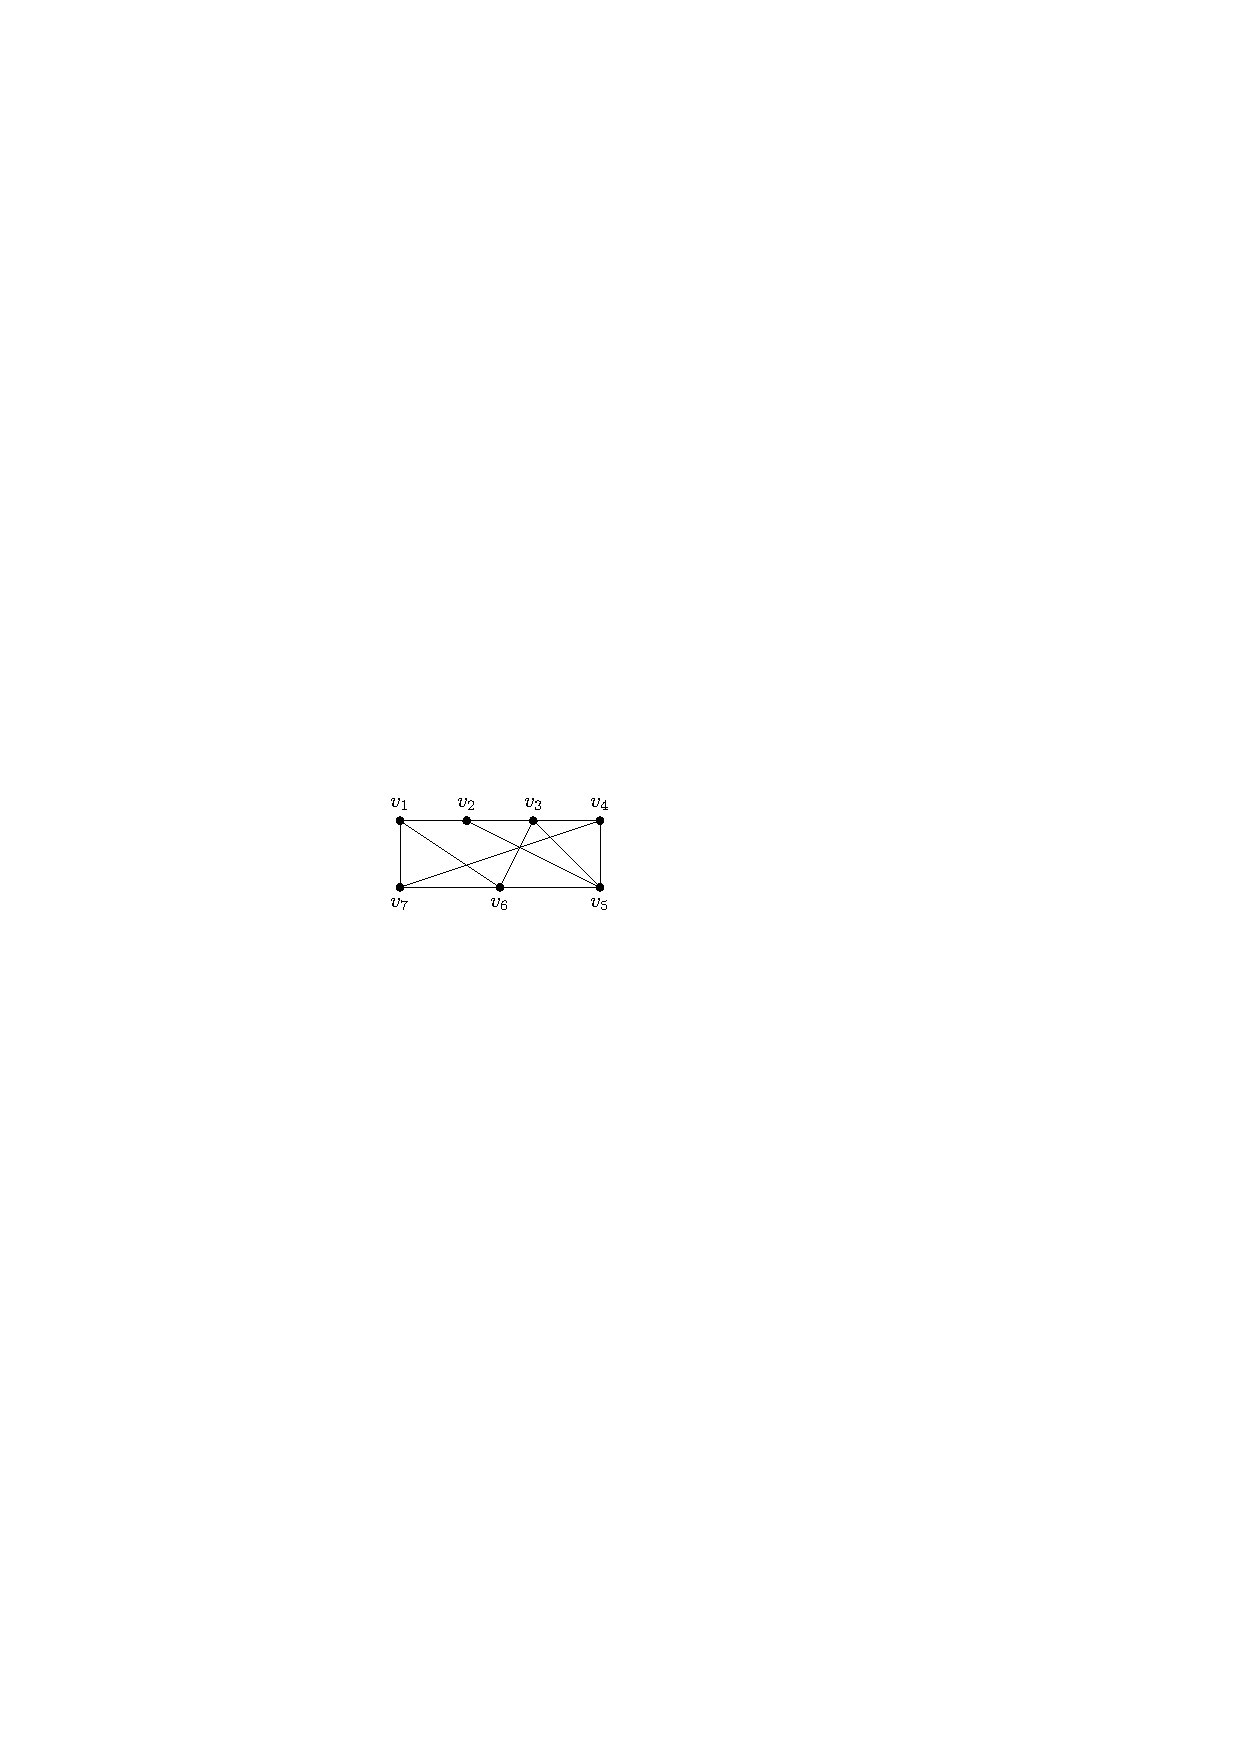
\includegraphics{Images/Subgraphs-G.pdf}} \hfill
\subcaptionbox{$H_1$\label{fig:SubgraphsH1}}{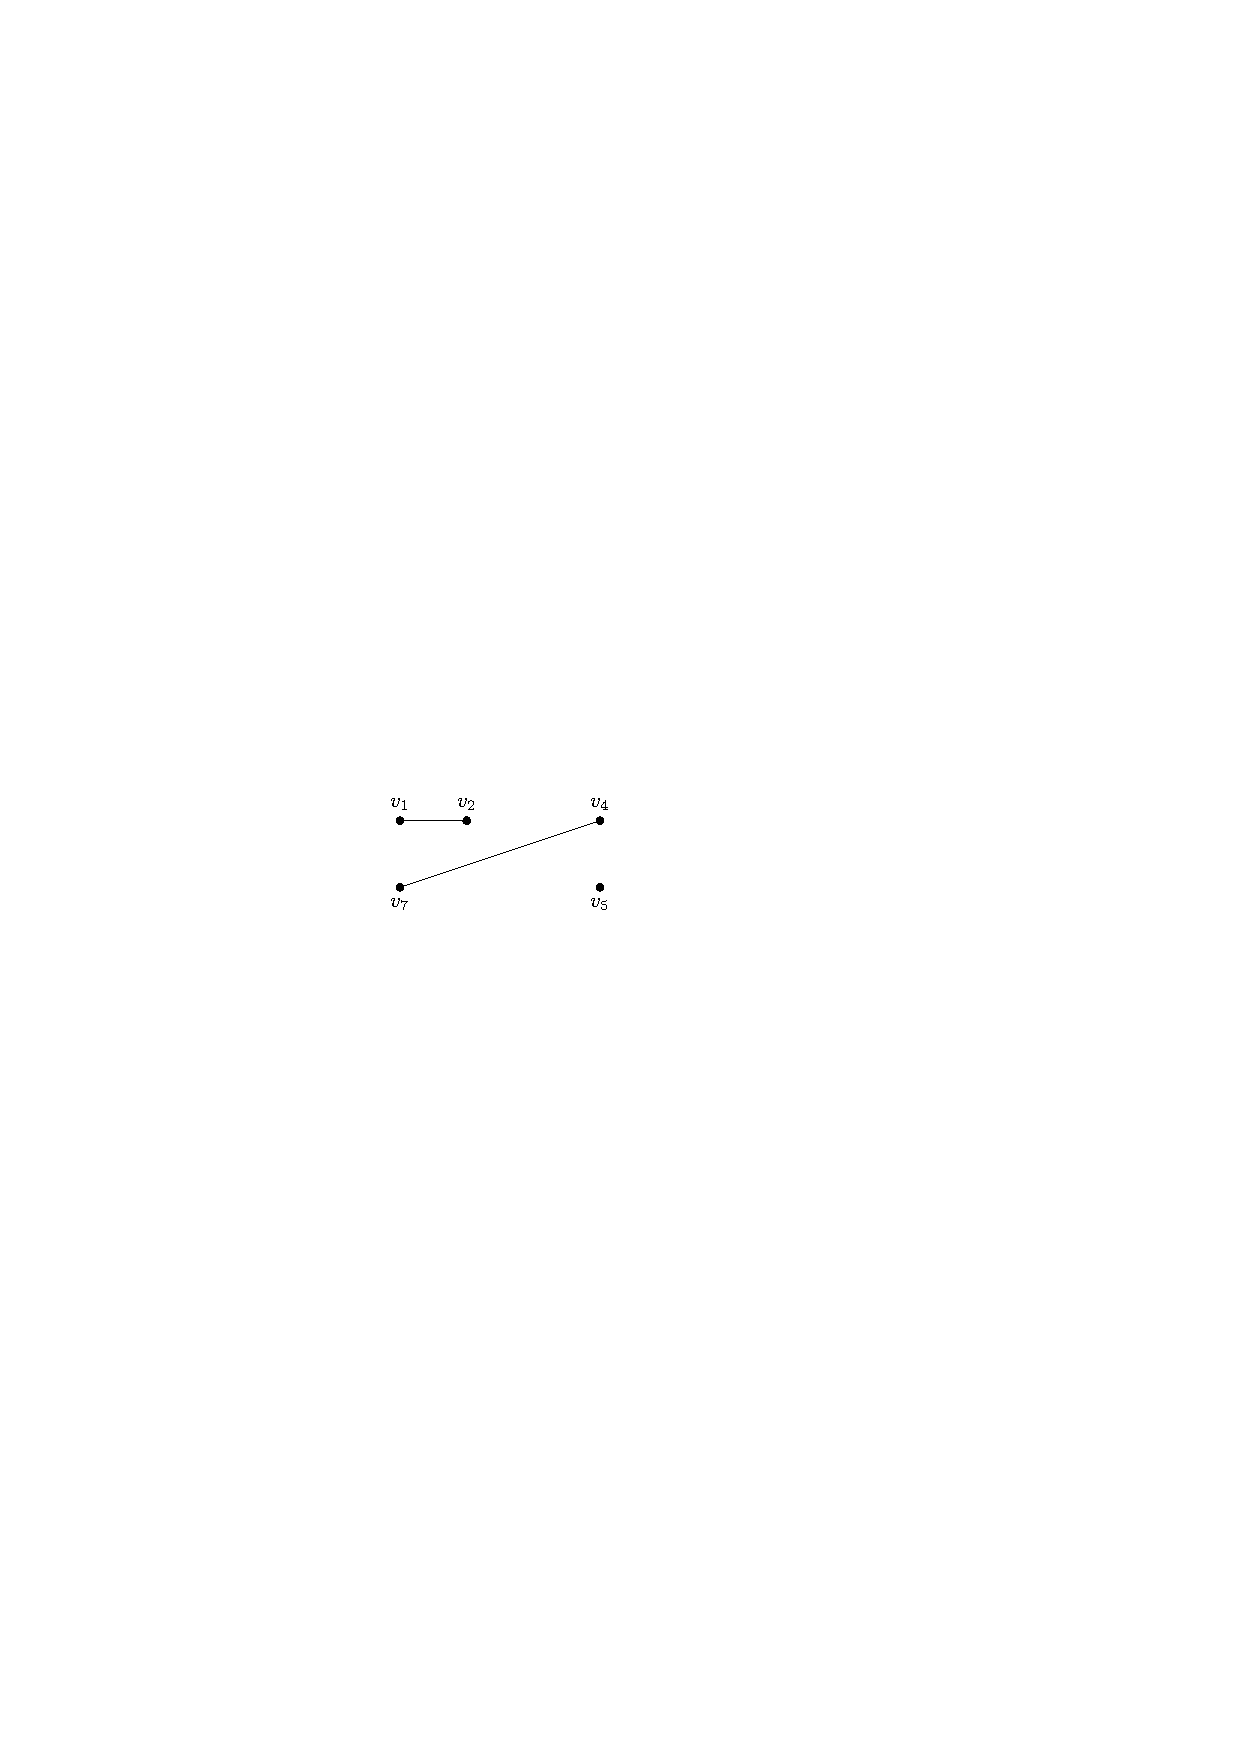
\includegraphics{Images/Subgraphs-H1.pdf}} \hfill
\subcaptionbox{$H_2$\label{fig:SubgraphsH2}}{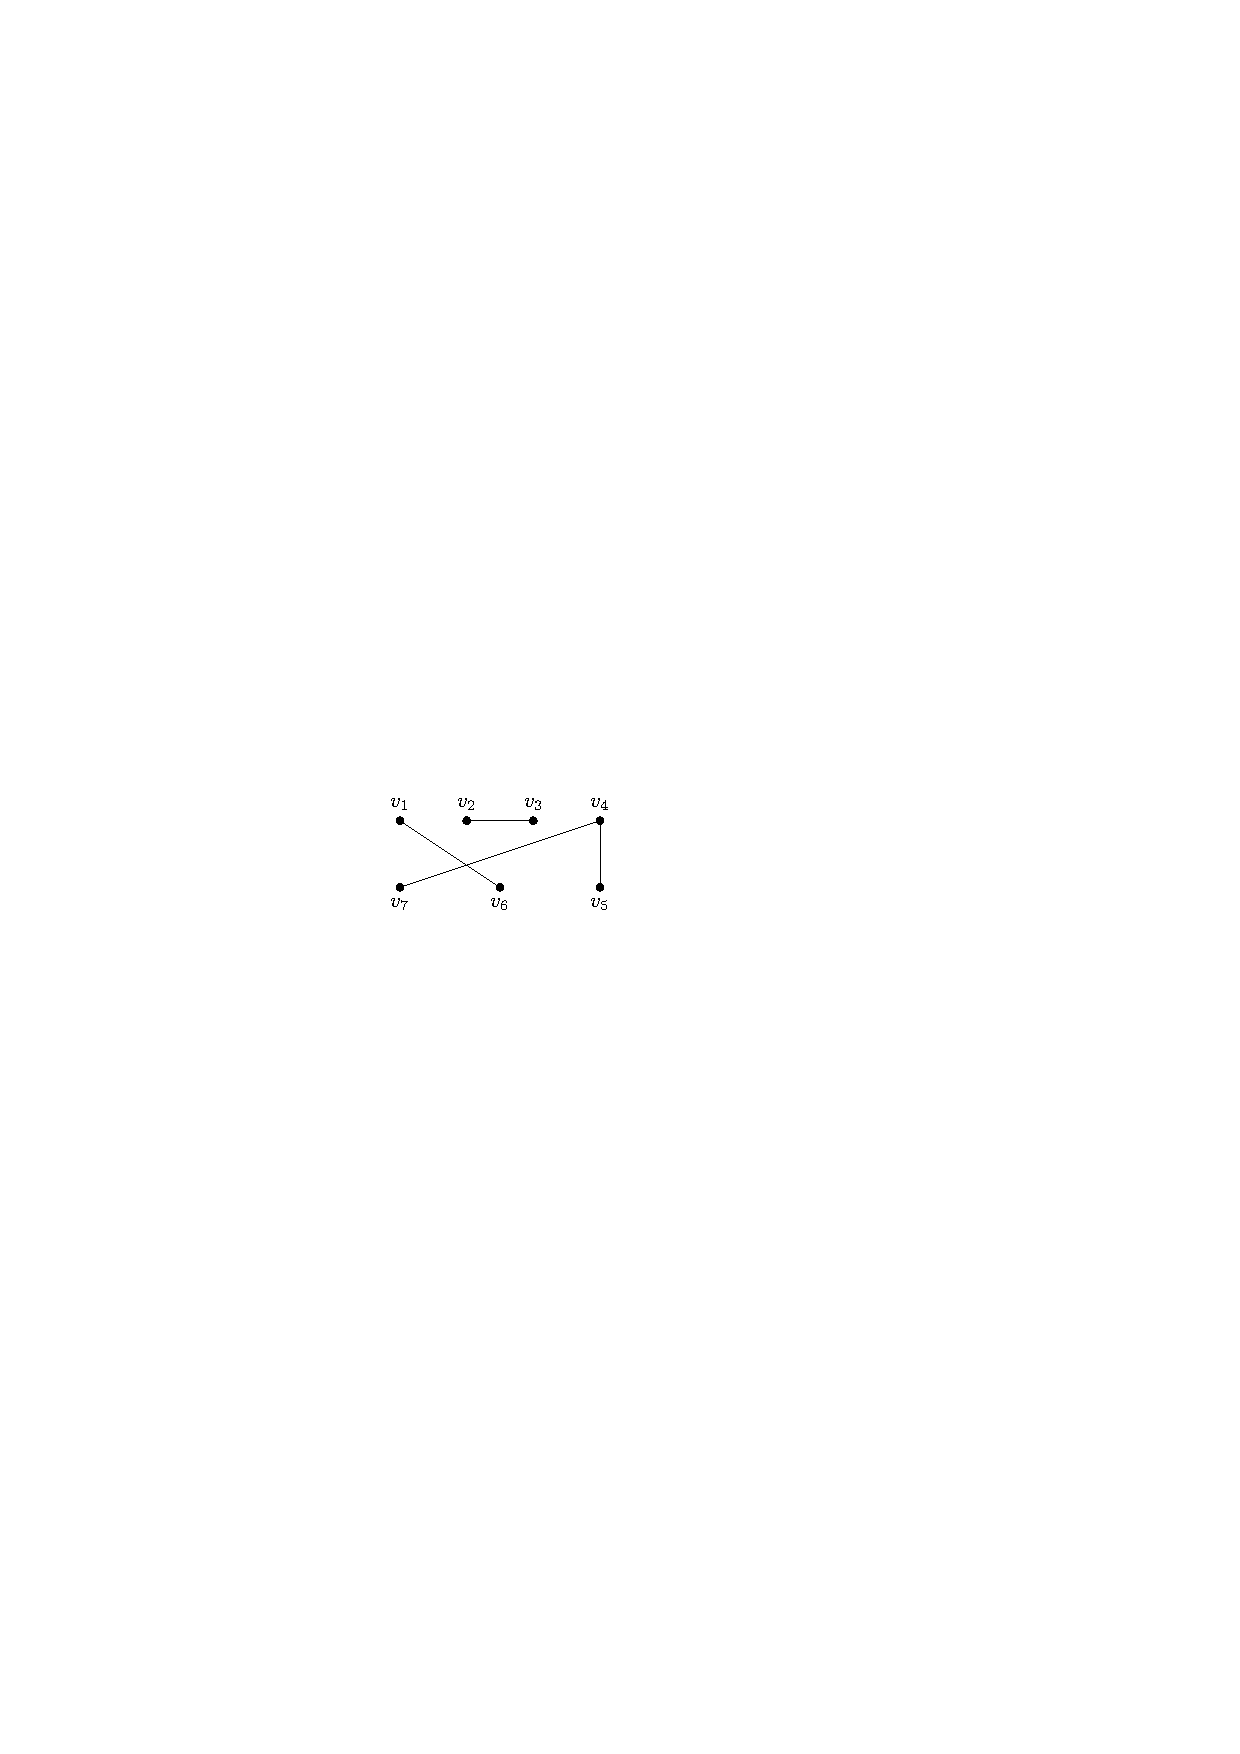
\includegraphics{Images/Subgraphs-H2.pdf}} \hfill
\subcaptionbox{$H_3$\label{fig:SubgraphsH3}}{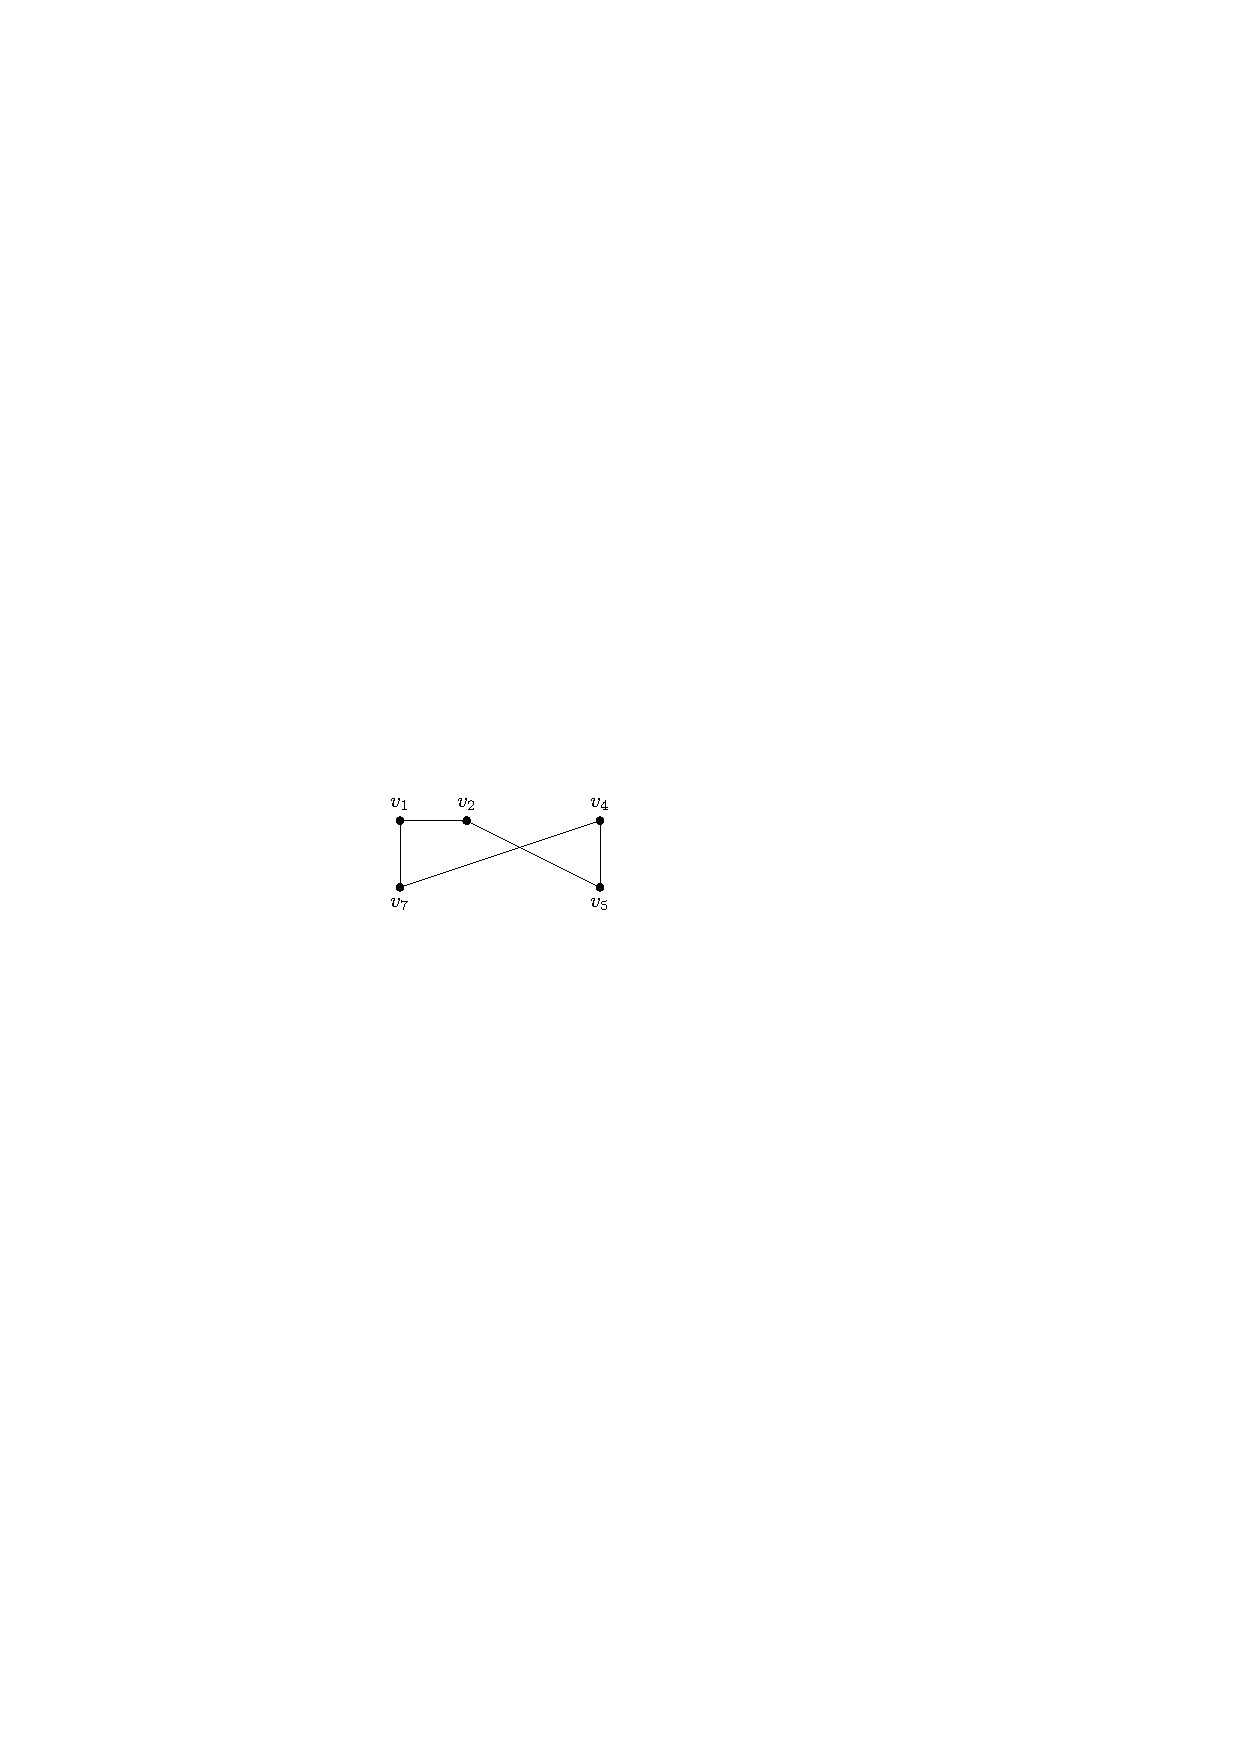
\includegraphics{Images/Subgraphs-H3.pdf}}
\caption{A graph with three of its subgraphs}\label{fig:Subgraphs}
\end{figure}
\end{Example}

A graph is \newterm{complete} if all its vertices are adjacent to one another. The complete graph of order $n$ is denoted by $K_n$. As there is an edge between every pair of distinct vertices of $K_n$, the size of $K_n$ is $\binom n 2$. A \newterm{totally disconnected graph} has no edges.

\subsection{Walks, Paths, and Cycles}\label{subsec:Walks}

A \newterm{walk} in a simple graph $G$ is a sequence of vertices $v_1, v_2, \ldots, v_k$ such that $v_i \sim v_{i + 1}$ for $i = 1, 2, \ldots, k - 1$. This is a walk \newterm{from $v_1$ to $v_k$} or \newterm{between $v_1$ and $v_k$}, having \newterm{length} $k - 1$. We may also say that this is a walk of length $k - 1$ starting at $v_1$ and ending at $v_k$.

A walk in which no vertex is repeated is a \newterm{path}. Note that the length of a path is the number of edges in it.

A \newterm{closed walk} in $G$ is a walk starting and ending at the same vertex. A closed walk in which no vertex is repeated (except for the start and end vertices being the same) is a \newterm{cycle}. The length of a cycle is also equal to the number of vertices in it. A cycle of the form $v_1, \ldots, v_{k-1}, v_k$ is usually referred to as ``the cycle $v_1, \ldots, v_{k-1}$''.

\begin{Example}\label{ex:Walk}
Consider the graph $G$ shown below.

\begin{center}
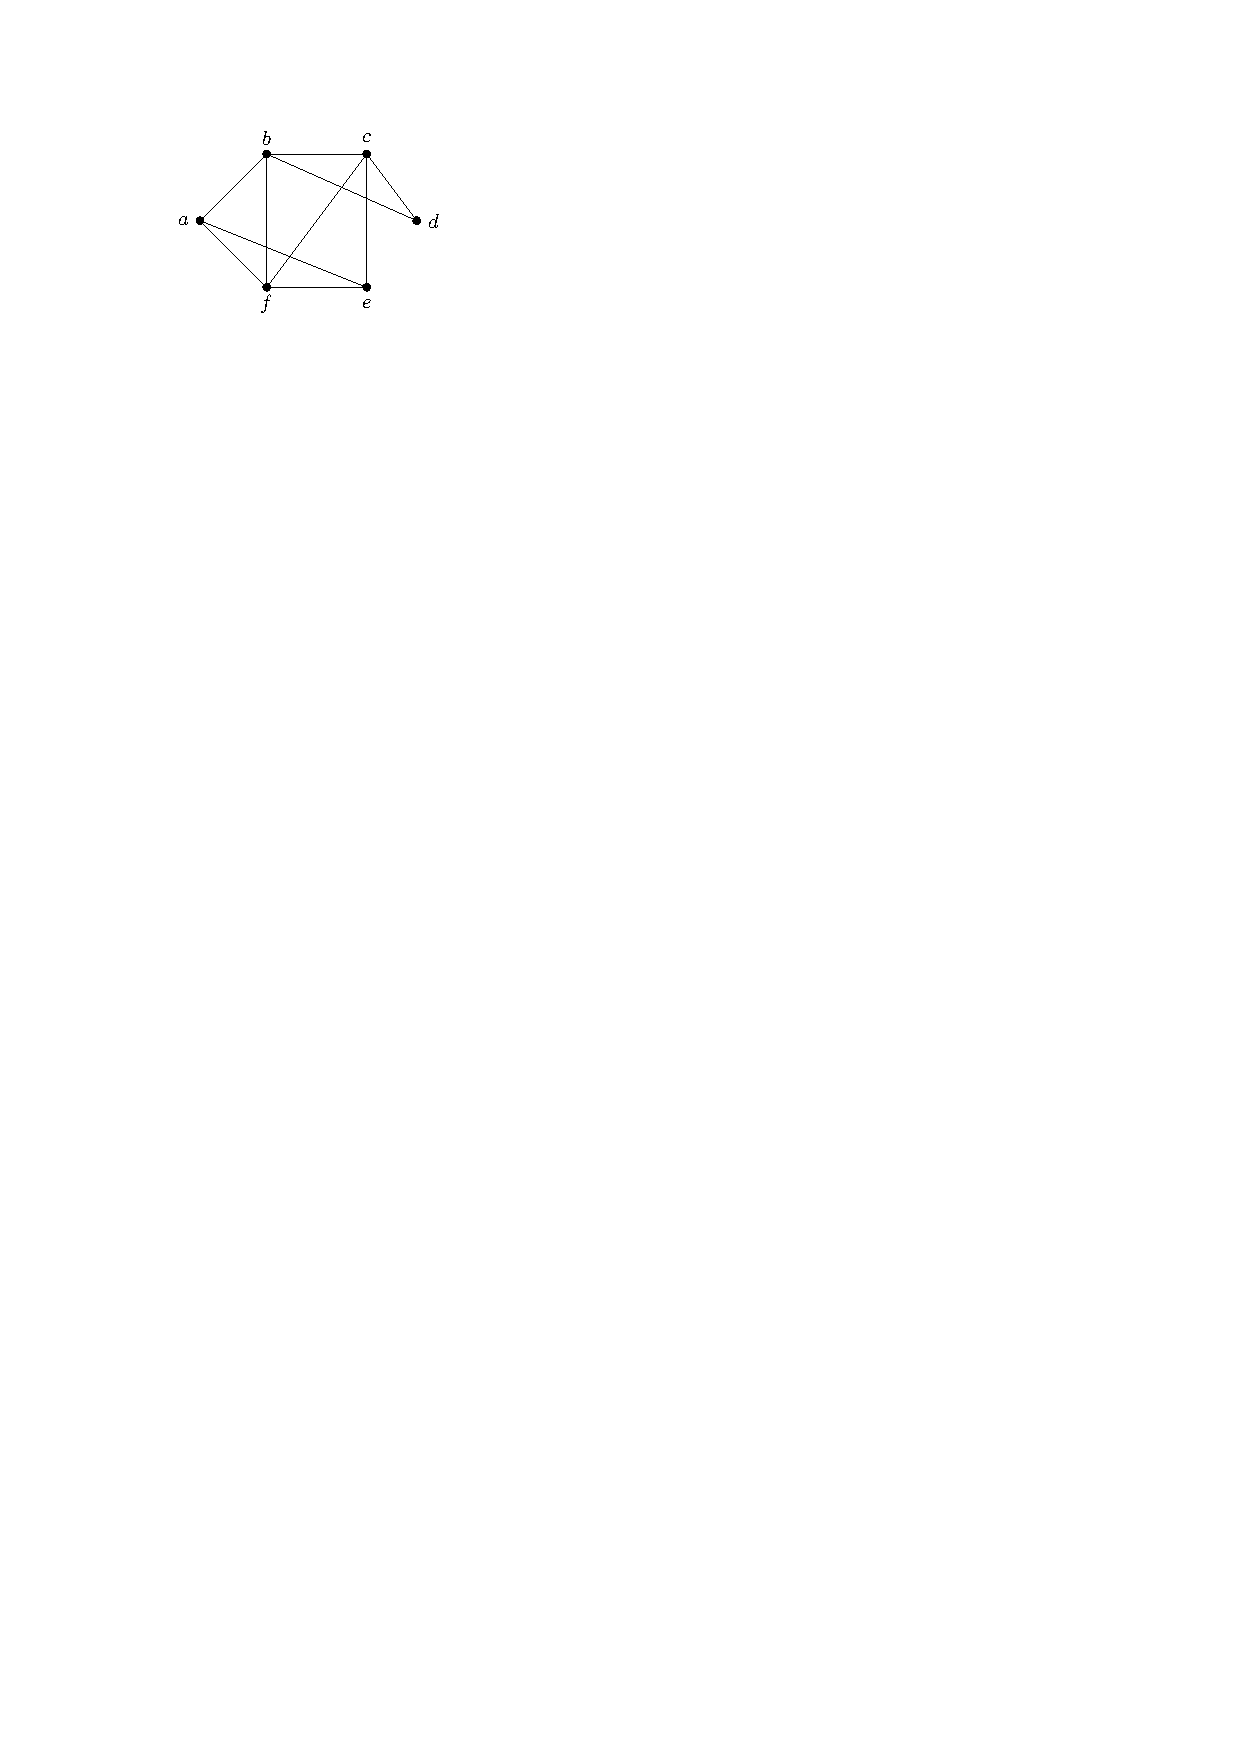
\includegraphics{Images/Walks.pdf}
\end{center}
A walk of length $5$ from $b$ to $c$ in $G$ is $b, f, e, a, e, c$.

\begin{center}
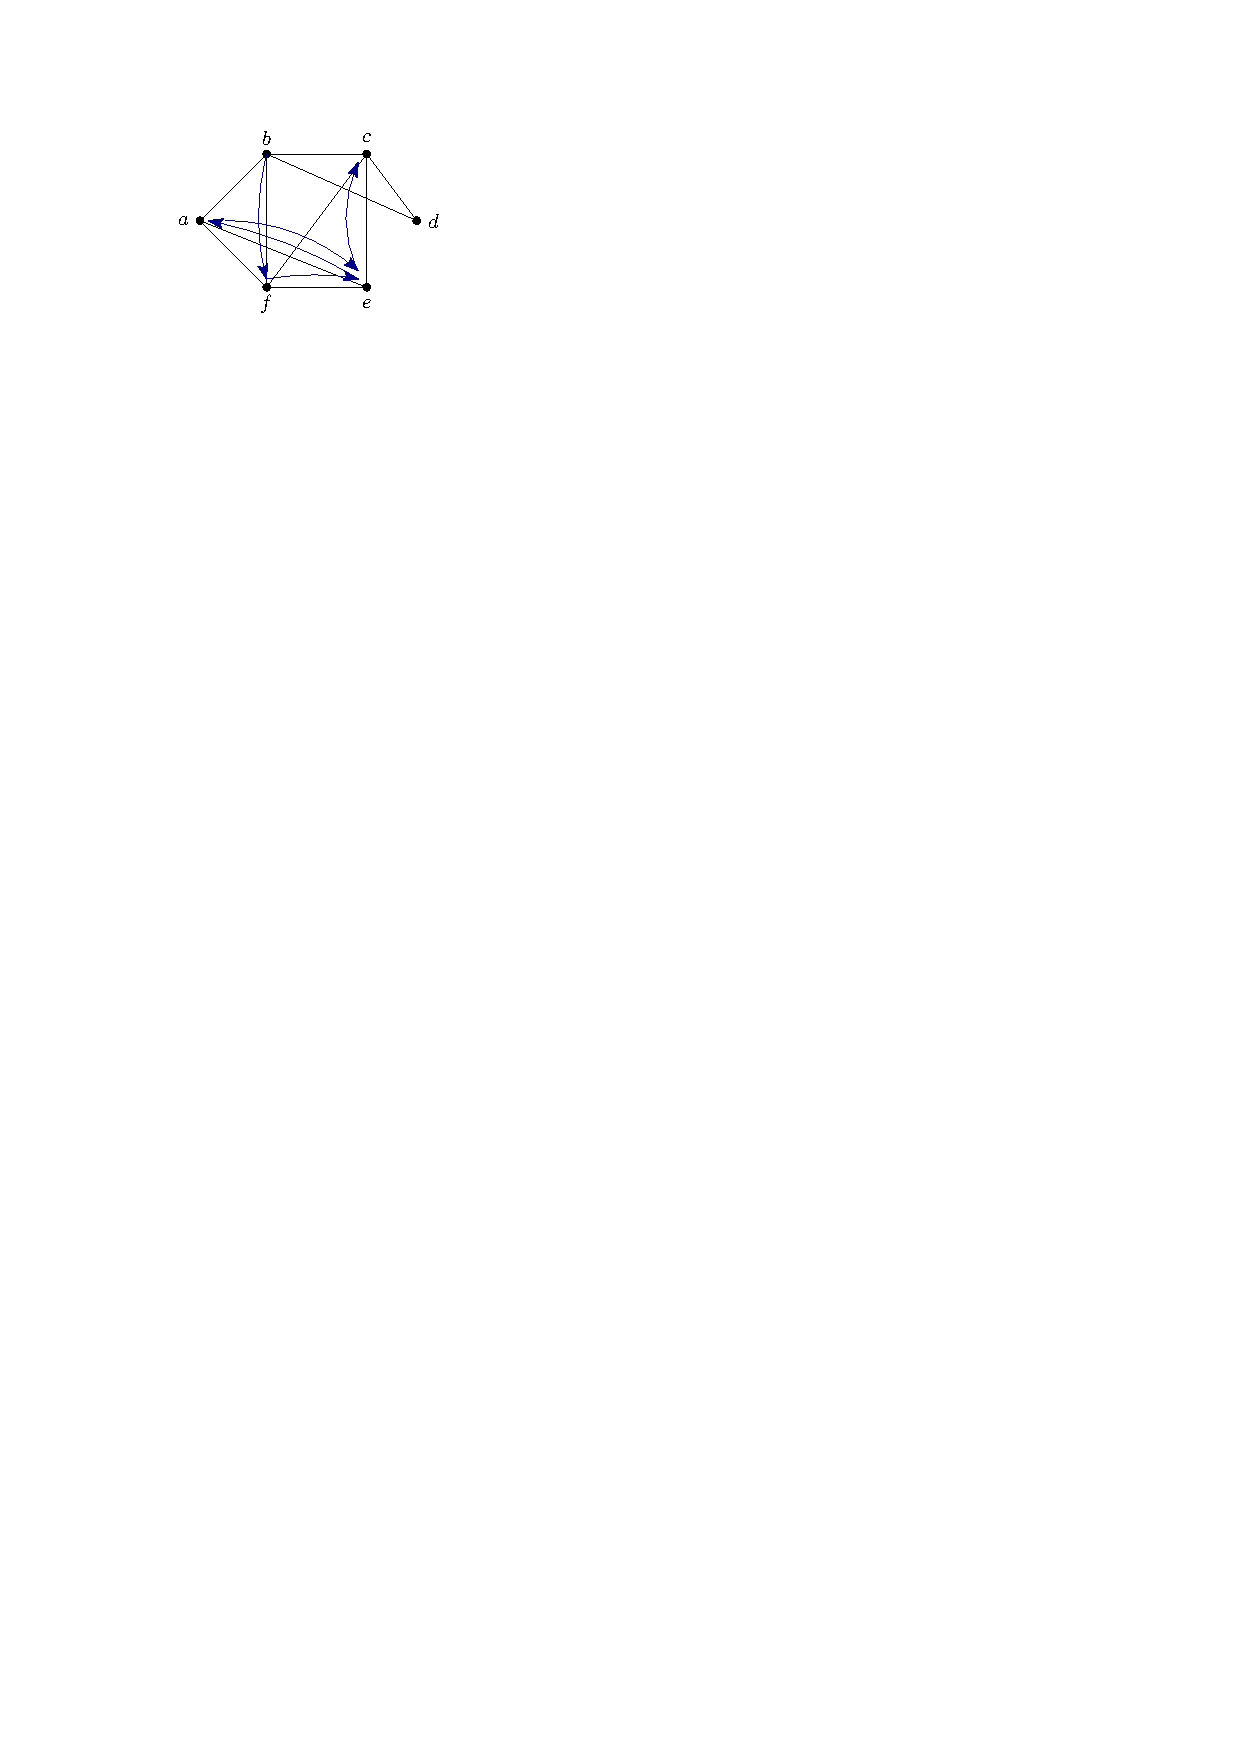
\includegraphics{Images/Walk1.pdf}
\end{center}
This walk is not a path, since the vertex $e$ is repeated. An example of a path from $b$ to $c$ in the same graph $G$ is $b, f, e, c$. The length of this path is $3$.

\begin{center}
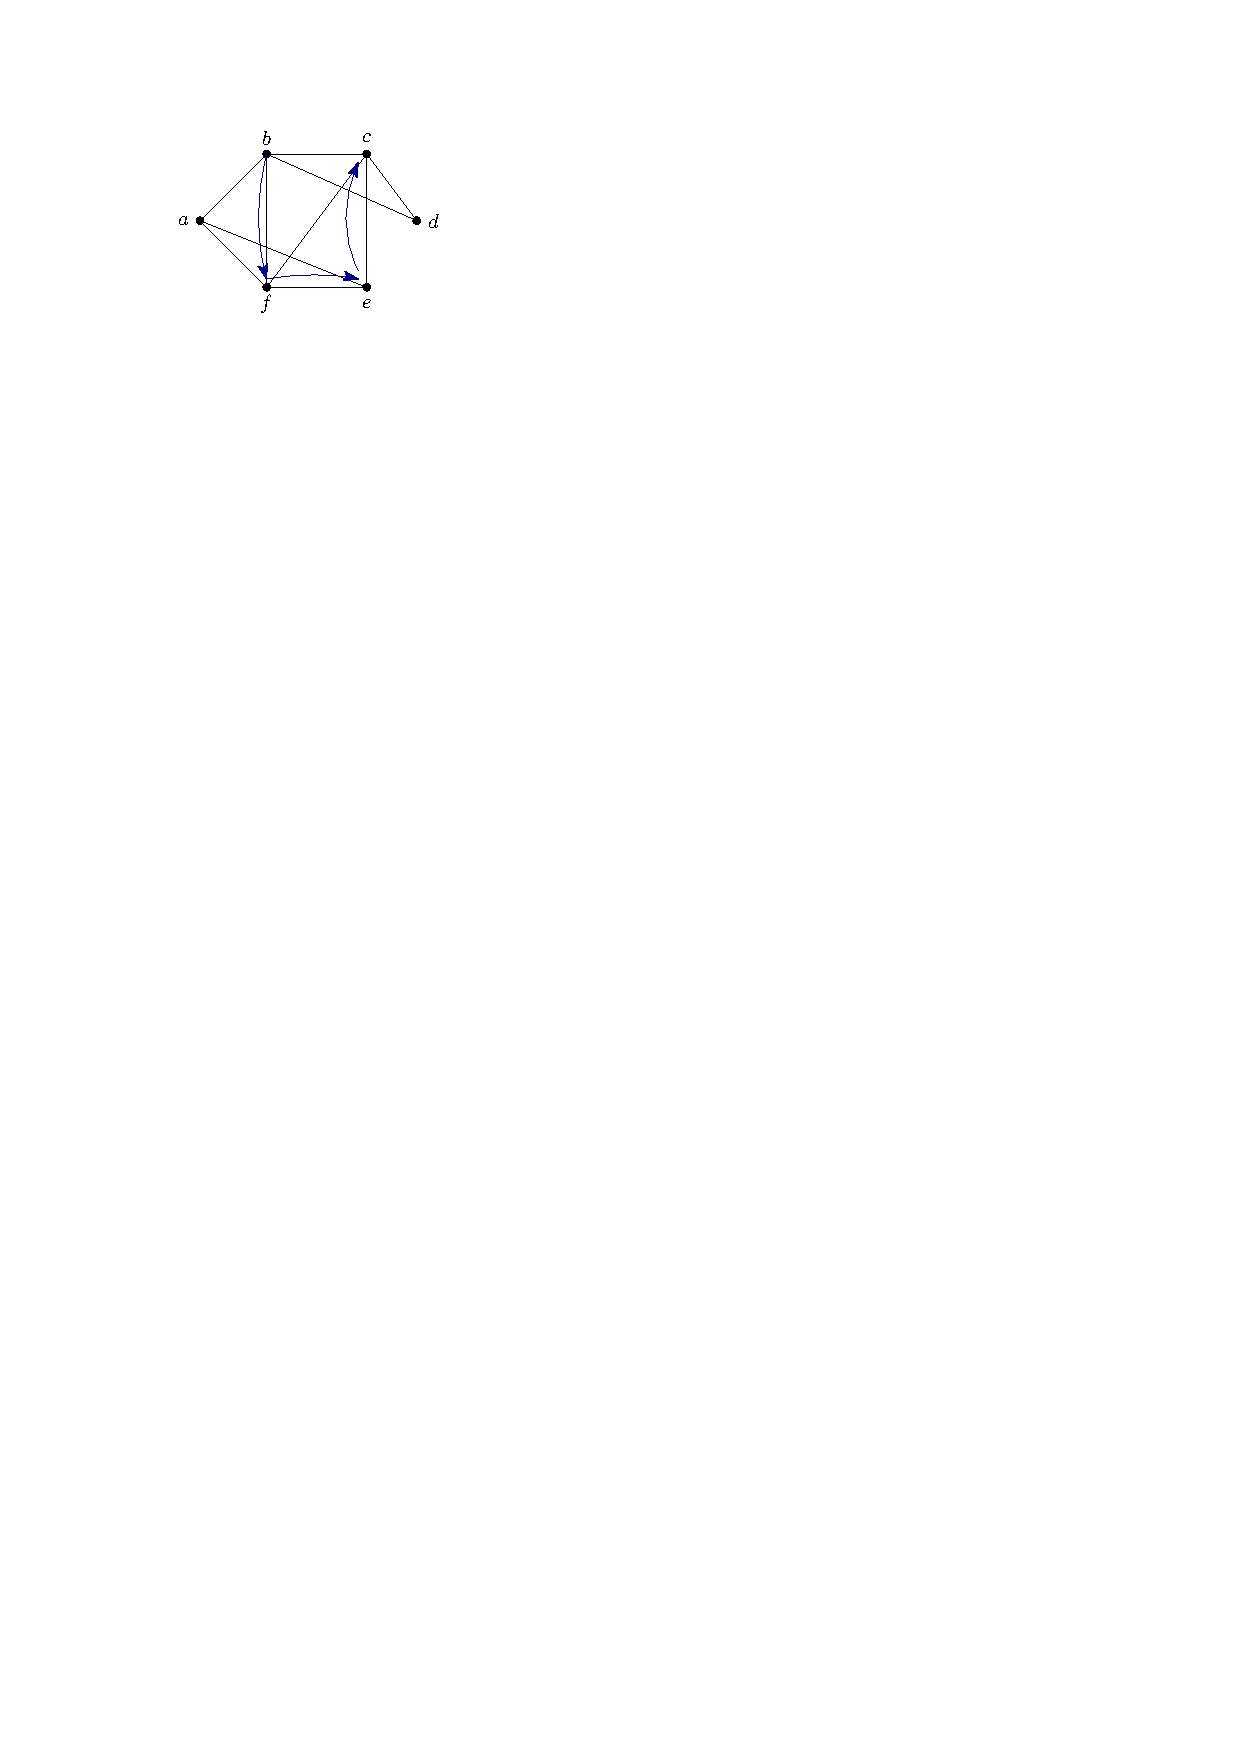
\includegraphics{Images/Path1.pdf}
\end{center}
A cycle of length $4$ in $G$ is $b, f, e, c, b$.

\begin{center}
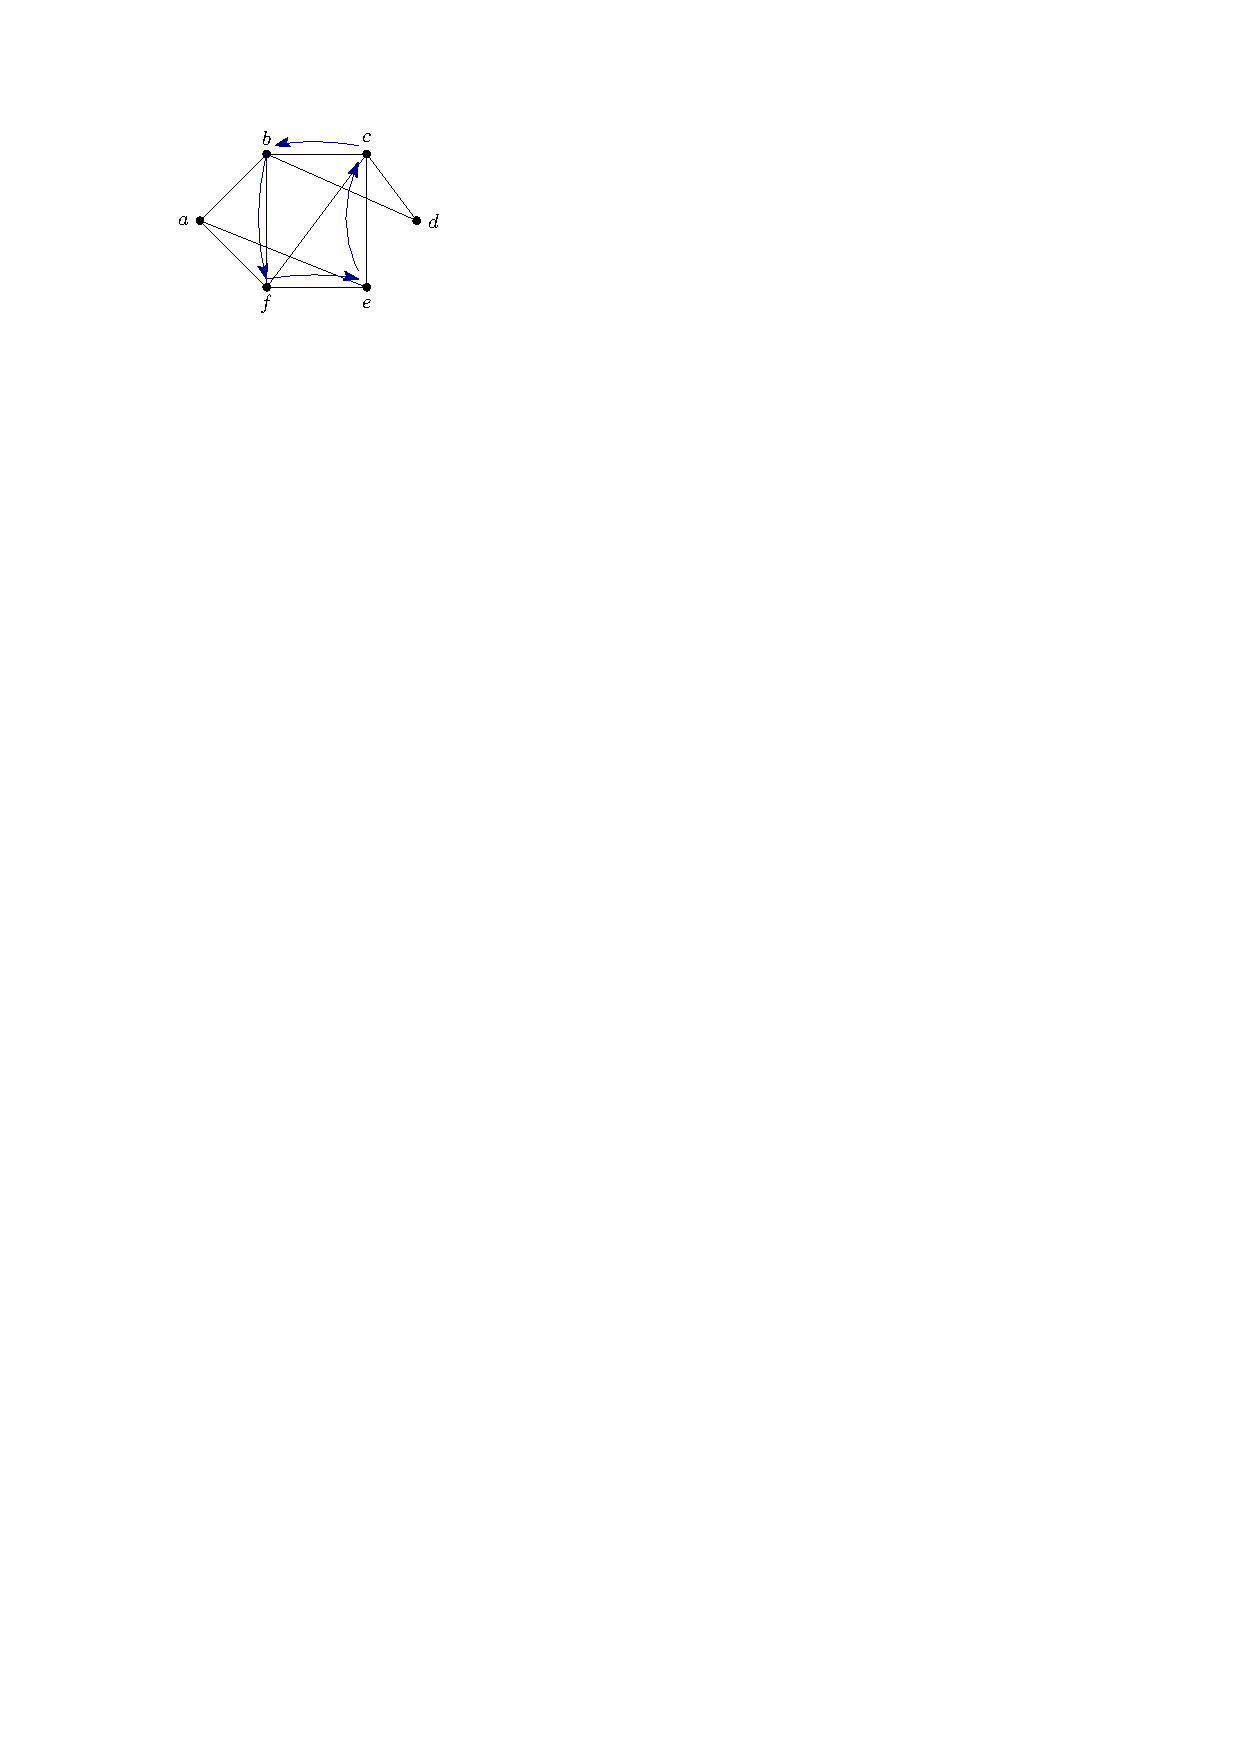
\includegraphics{Images/Cycle1.pdf}
\end{center}
\end{Example}

\begin{Theorem}\label{thm:deltaGPath}
If $\delta(G) \ge 2$, then $G$ contains a path of length $\delta(G)$ and a cycle of length greater than $\delta(G)$.
\end{Theorem}

\begin{proof}
Let $P = v_0 v_1 \cdots v_k$ be a longest path in $G$. Then all the neighbours of $v_0$ must be on $P$ (for otherwise, we would get a path longer than $P$). Hence, $k \ge \deg v_0 \ge \delta(G)$, so $P$ has length at least $\delta(G)$.

Next, let $i \le k$ be maximal such that $v_i \sim v_0$. Since all $\deg v_0$ neighbours of $v_0$ occur among $v_1,\ldots,v_i$, we have $i \ge \deg v_0 \ge \delta(G)$. Therefore, $v_0 v_1 \cdots v_i v_0$ is a cycle of length $i + 1 > \delta(G)$.
\end{proof}

\begin{Exercise}
Prove that any two longest paths in a connected graph share at least one common vertex.
\end{Exercise}

\subsection{Distances and Connectedness}\label{subsec:DistancesConnectedness}

The \newterm{distance} between two vertices $u$ and $v$ of a graph $G$ is the length of a shortest path between $u$ and $v$ -- such a shortest path between $u$ and $v$ is a \newterm{geodesic} from $u$ to $v$. Thus, the distance between $u$ and $v$ in $G$, denoted by $d_G(u, v)$, is the length of a geodesic from $u$ to $v$ in $G$. If there is no path from $u$ to $v$ in $G$, then we set $d_G(u, v) = \infty$. When the graph $G$ is clear from the context, we will write $d_G(u, v)$ as $d(u, v)$.

A graph is \newterm{connected} if there is a path between every two of its vertices. Otherwise, it is \newterm{disconnected}. A \newterm{(connected) component} of a graph $G$ is a maximal connected subgraph of $G$. Thus, a graph $G$ is connected if and only if it has exactly one component.

The \newterm{eccentricity} of a vertex $v$, denoted by $\ecc(v)$, is the maximum of all distances from $v$ to any other vertex. That is,
\begin{equation*}
    \ecc(v) = \max_{u \in V(G)} d(u, v) .
\end{equation*}

The \newterm{diameter} of $G$ is the maximum of the eccentricities of vertices of $G$, and the \newterm{radius} of $G$ is the minimum of the eccentricities of vertices of $G$. They are denoted by $\diam(G)$ and $\rad(G)$ respectively. Thus,
\begin{align*}
    \diam(G) & = \max_{v \in V(G)} \ecc(v)= \max_{u, v \in V(G)} d(u, v) \\
    \rad(G) & = \min_{v \in V(G)}\ecc(v) = \min_{v \in V(G)} \max_{u \in V(G)} d(u, v).
\end{align*}

The set of all vertices of $G$ having minimum eccentricity,i.e.\ the set of all $v \in V(G)$ such that $\ecc v = \rad G$, is the \newterm{centre} of $G$.

\begin{Exercise}
Prove that for any connected graph $G$, $\rad G \le \diam G \le 2 \rad G$.
\end{Exercise}


\subsection{Bipartite Graphs}\label{subsec:Bipartite}

A graph $G = (V, E)$ is \newterm{bipartite} if its vertex set $V$ can be partitioned into two (possibly empty) subsets $V_1$ and $V_2$ such that no two vertices in $V_i$ are adjacent, for $i = 1, 2$. That is, there exist two disjoint subsets $V_1, V_2 \subseteq V$ such that $V_1 \cup V_2 = V$, and every edge of $G$ (if any) joins a vertex in $V_1$ with a vertex in $V_2$. Then we say that $(V_1, V_2)$ is a \newterm{bipartition} of $G$.

The following theorem characterises bipartite graphs in terms of their cycles. A cycle is \newterm{even} if its length is even and \newterm{odd} if its length is odd.

\begin{Theorem}
A graph is bipartite if and only if it contains no odd cycles.
\end{Theorem}

The \newterm{complete bipartite graph} $K_{m,n}$ is the bipartite graph with $m$ vertices in one partite set and $n$ vertices in the other partite set, such that every vertex of one partite set is adjacent to every vertex of the other.

\subsection{Trees}\label{subsec:Trees}

A \newterm{tree} is a connected, acyclic graph. There are several well-known characterisations or alternative definitions of trees. We take the given definition as the basic one and prove its equivalence to some others. If $u$ and $v$ are non-adjacent vertices of a graph $T$, then $T+uv$ denotes the graph obtained from $T$ by adding the edge $uv$.

\begin{Theorem}\label{thm:Conn;p=q+1}
If $T$ is a graph of order $p$ and size $q$, the following are equivalent:
\begin{enumerate}[label =(\roman*)]
\item $T$ is a tree.
\item Any two vertices of $T$ are joined by a unique path.
\item $T$ is connected and $p = q + 1$.
\item $T$ is acyclic and $p = q + 1$.
\item $T$ is connected and for any edge $e$ of $T$, $T - e$ is disconnected.
\item $T$ is acyclic and for any two non-adjacent vertices $u$ and $v$ of $T$, $T + uv$ contains a unique cycle.
\item $T$ is connected and either of order at most $2$, or not complete, and for any two non-adjacent vertices $u$ and $v$ of $T$, $T + uv$ contains a unique cycle. 
\end{enumerate}
\end{Theorem}


\begin{Exercise}
A \newterm{pendant vertex} of a graph is a vertex of degree $1$. Prove that every non-trivial tree contains at least two pendant vertices.\\
    \hint{If a tree of order $p\ge 2$ had at most one vertex of degree $1$, its degree sum would be at least $1+2(p-1)=2p-1$, contradicting the Handshaking Lemma and the fact that its size is $p-1$.}
\end{Exercise}

\begin{Exercise}
The \newterm{centre} of a graph $G$ is the set of all vertices of $G$ with minimum eccentricity -- i.e.\ the set of all vertices $v$ of $G$ with $\ecc v = \rad G$. Show that every tree has a centre consisting of either exactly one vertex or exactly two adjacent vertices.\\
\hint{Handle trees of orders $1$ and $2$ separately. Deleting all pendant vertices from a tree of order at least $3$ results in a smaller tree with the same centre.}
\end{Exercise}

% The following material is retained for Topics 2 and 3, but is not part of
% Topic 1. Remove the \iffalse and \fi when it is ready to be developed.
\iffalse
\subsection{Line Graphs}\label{subsec:LineGraphs}

Let $G$ be a graph with at least one edge. The \newterm{line graph} of $G$ is the graph $L(G)$ whose vertex set is the edge set of $G$, in which two vertices $e$ and $f$ are adjacent if the edges $e$ and $f$ of $G$ are adjacent.

\begin{Example}\label{ex:LineGrpahs}
\cref{fig:LineGraphs} shows a graph $G$ with eight edges and its line graph $L(G)$.
\begin{figure}[!htbp]
\centering
\subcaptionbox{$G$}{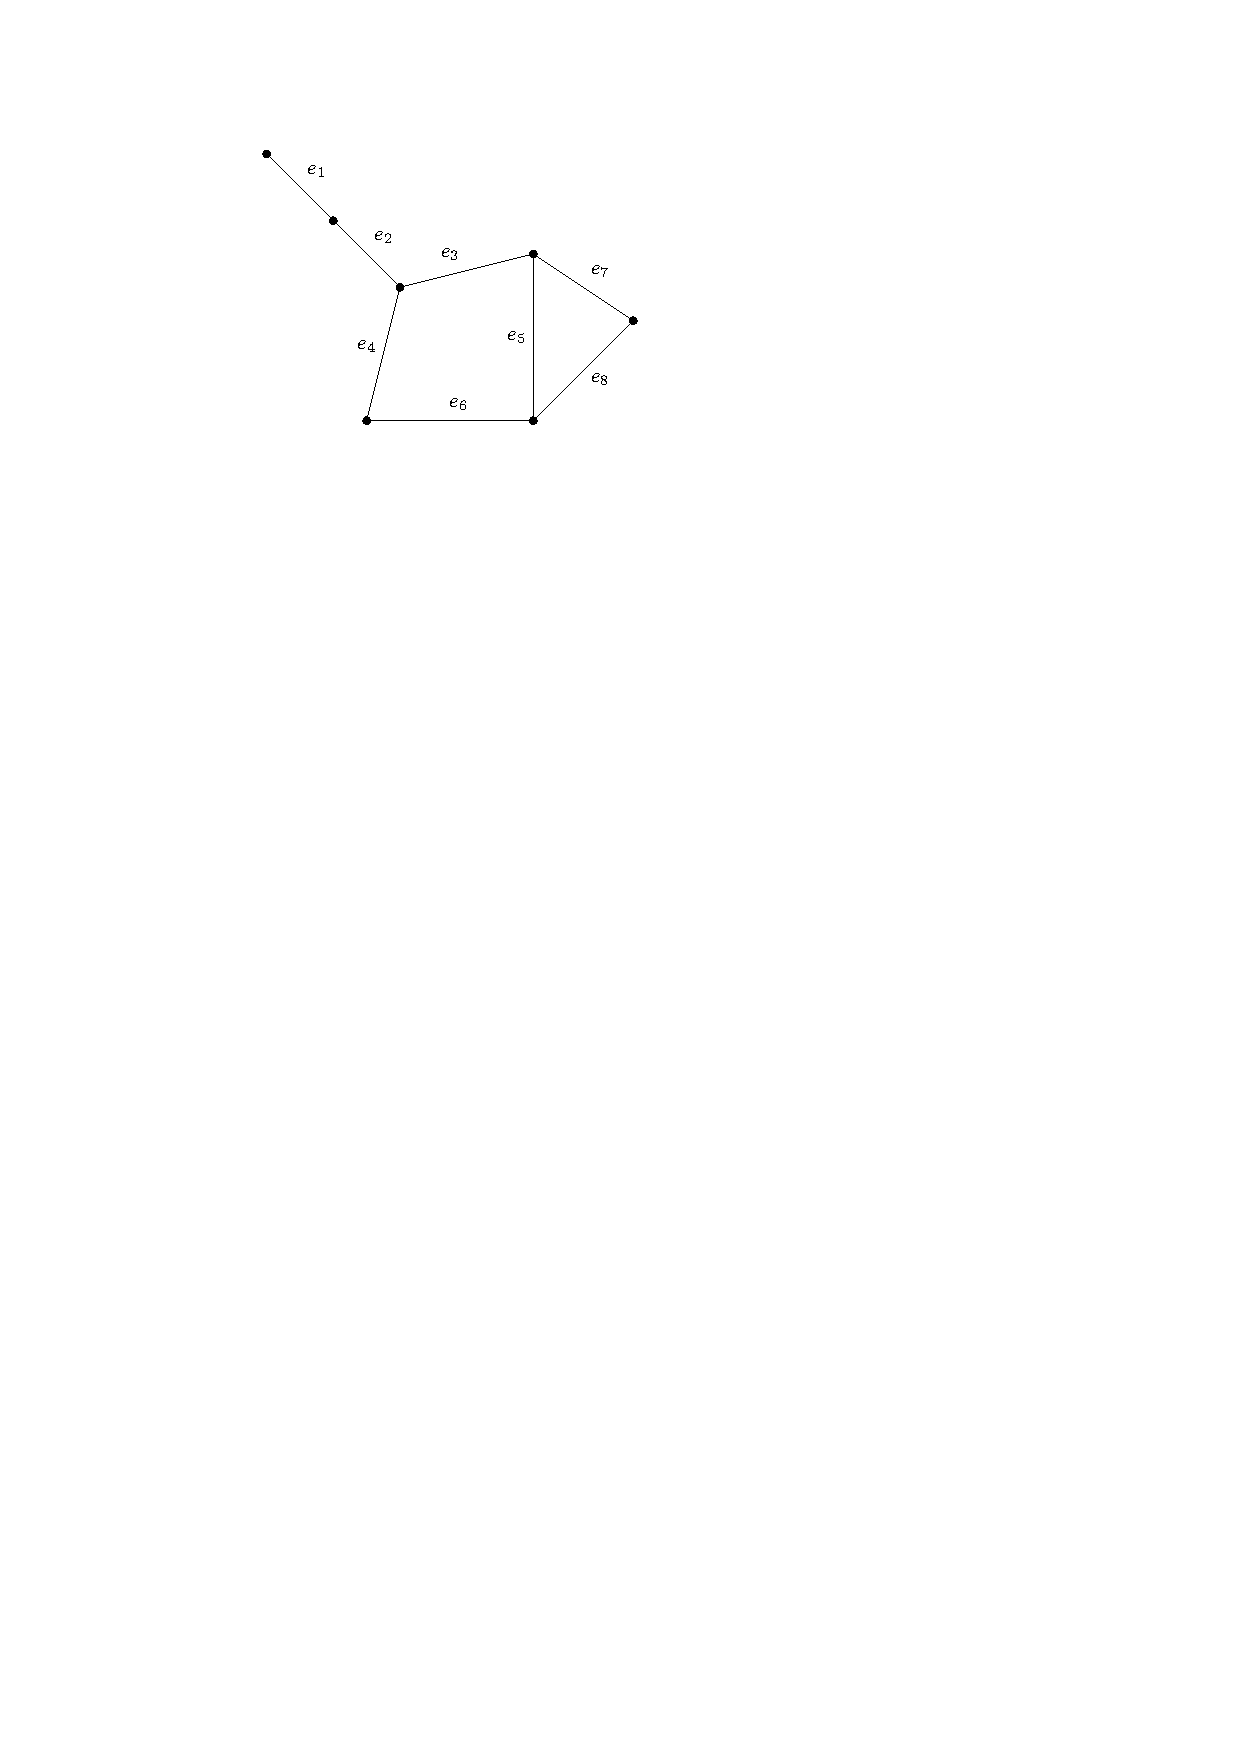
\includegraphics{Images/GNM(7,8).pdf}} \hspace{5em}
\subcaptionbox{$L(G)$}{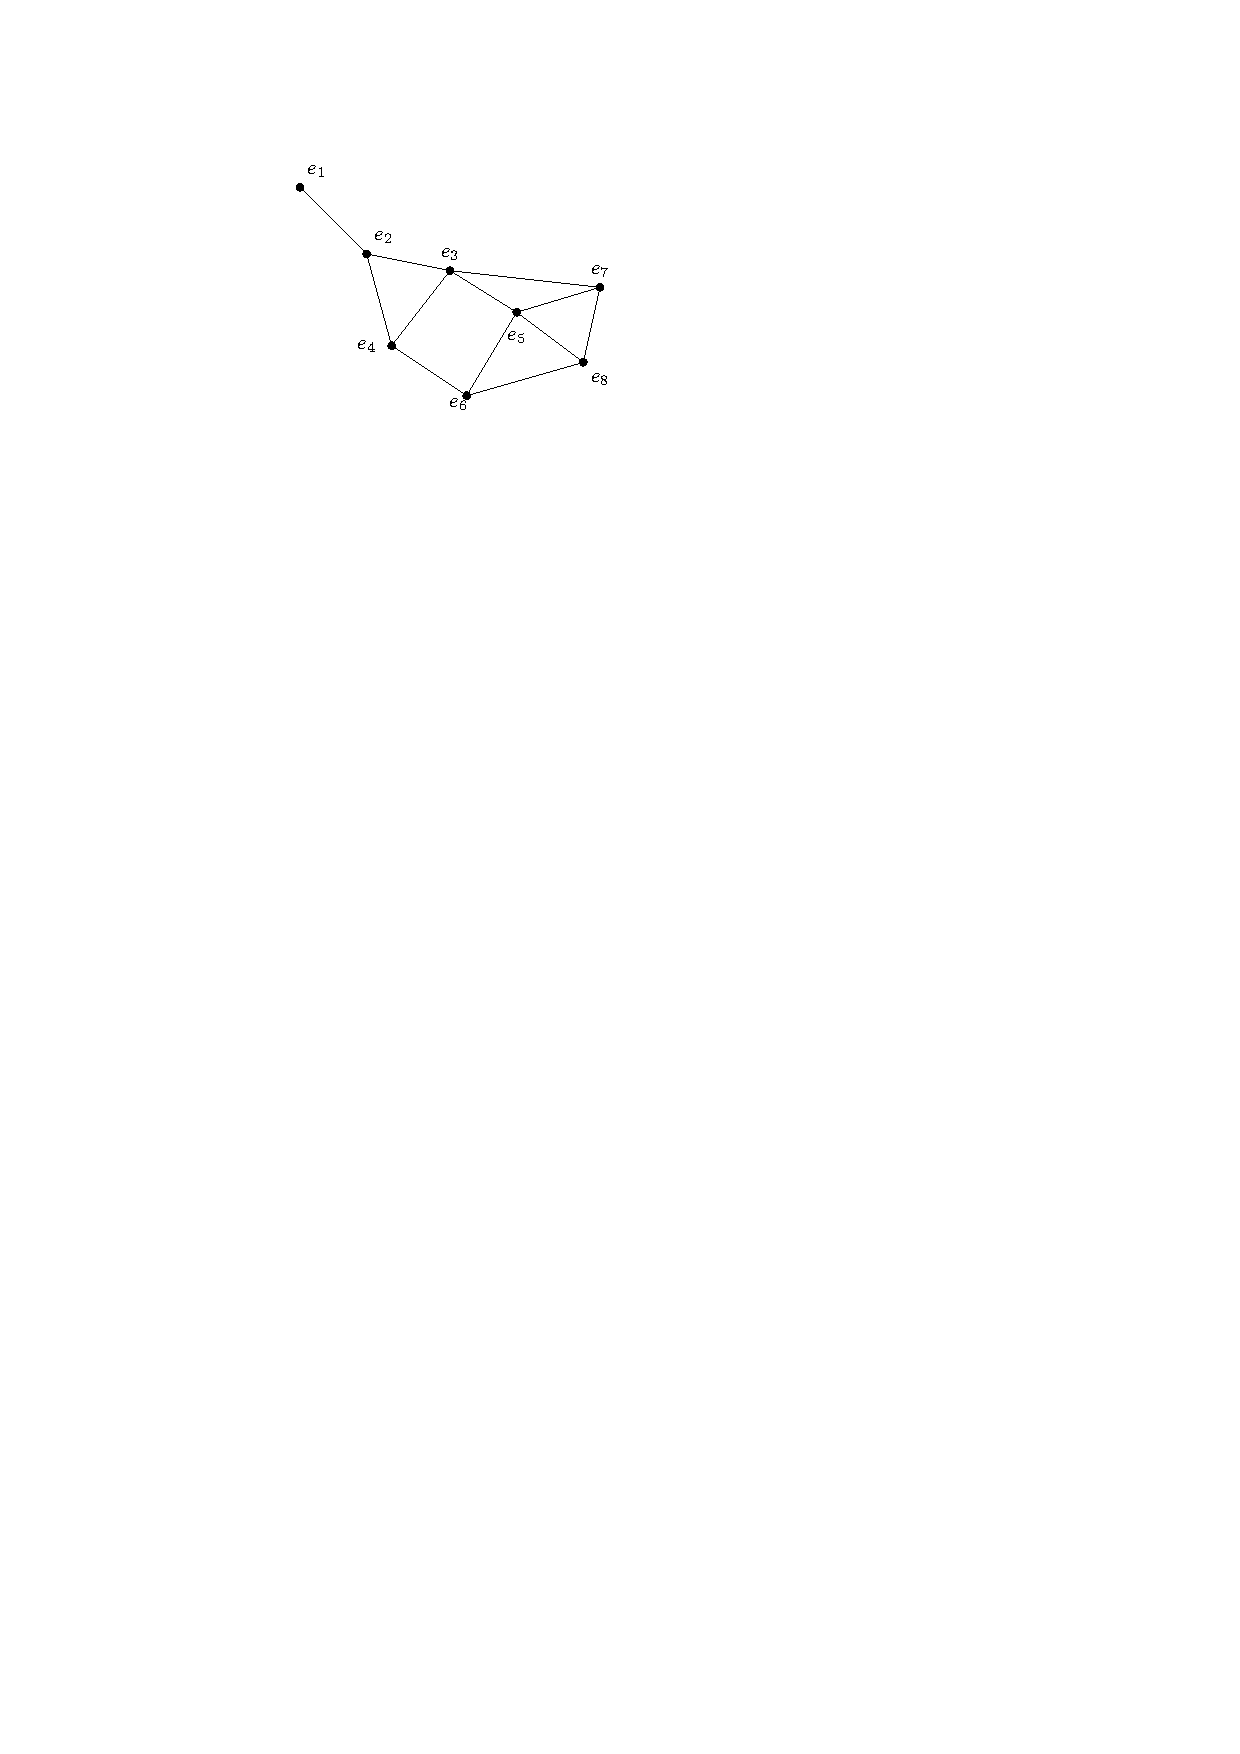
\includegraphics{Images/L(GNM(7,8)).pdf}}
\caption{A graph and its line graph}\label{fig:LineGraphs}
\end{figure}
\end{Example}

If $u$ and $v$ are edges joined by an edge $e$ in $G$, then in $L(G)$, the vertex $e$ will be adjacent to all the vertices corresponding to the edges of $G$ other than $e$ that are incident with $u$ and $v$ (see \cref{fig:L(G)Neighbourhood}). Thus, $\deg_{L(G)} e = \deg_G u + \deg_G v - 2$.
\begin{figure}[!htbp]
\centering
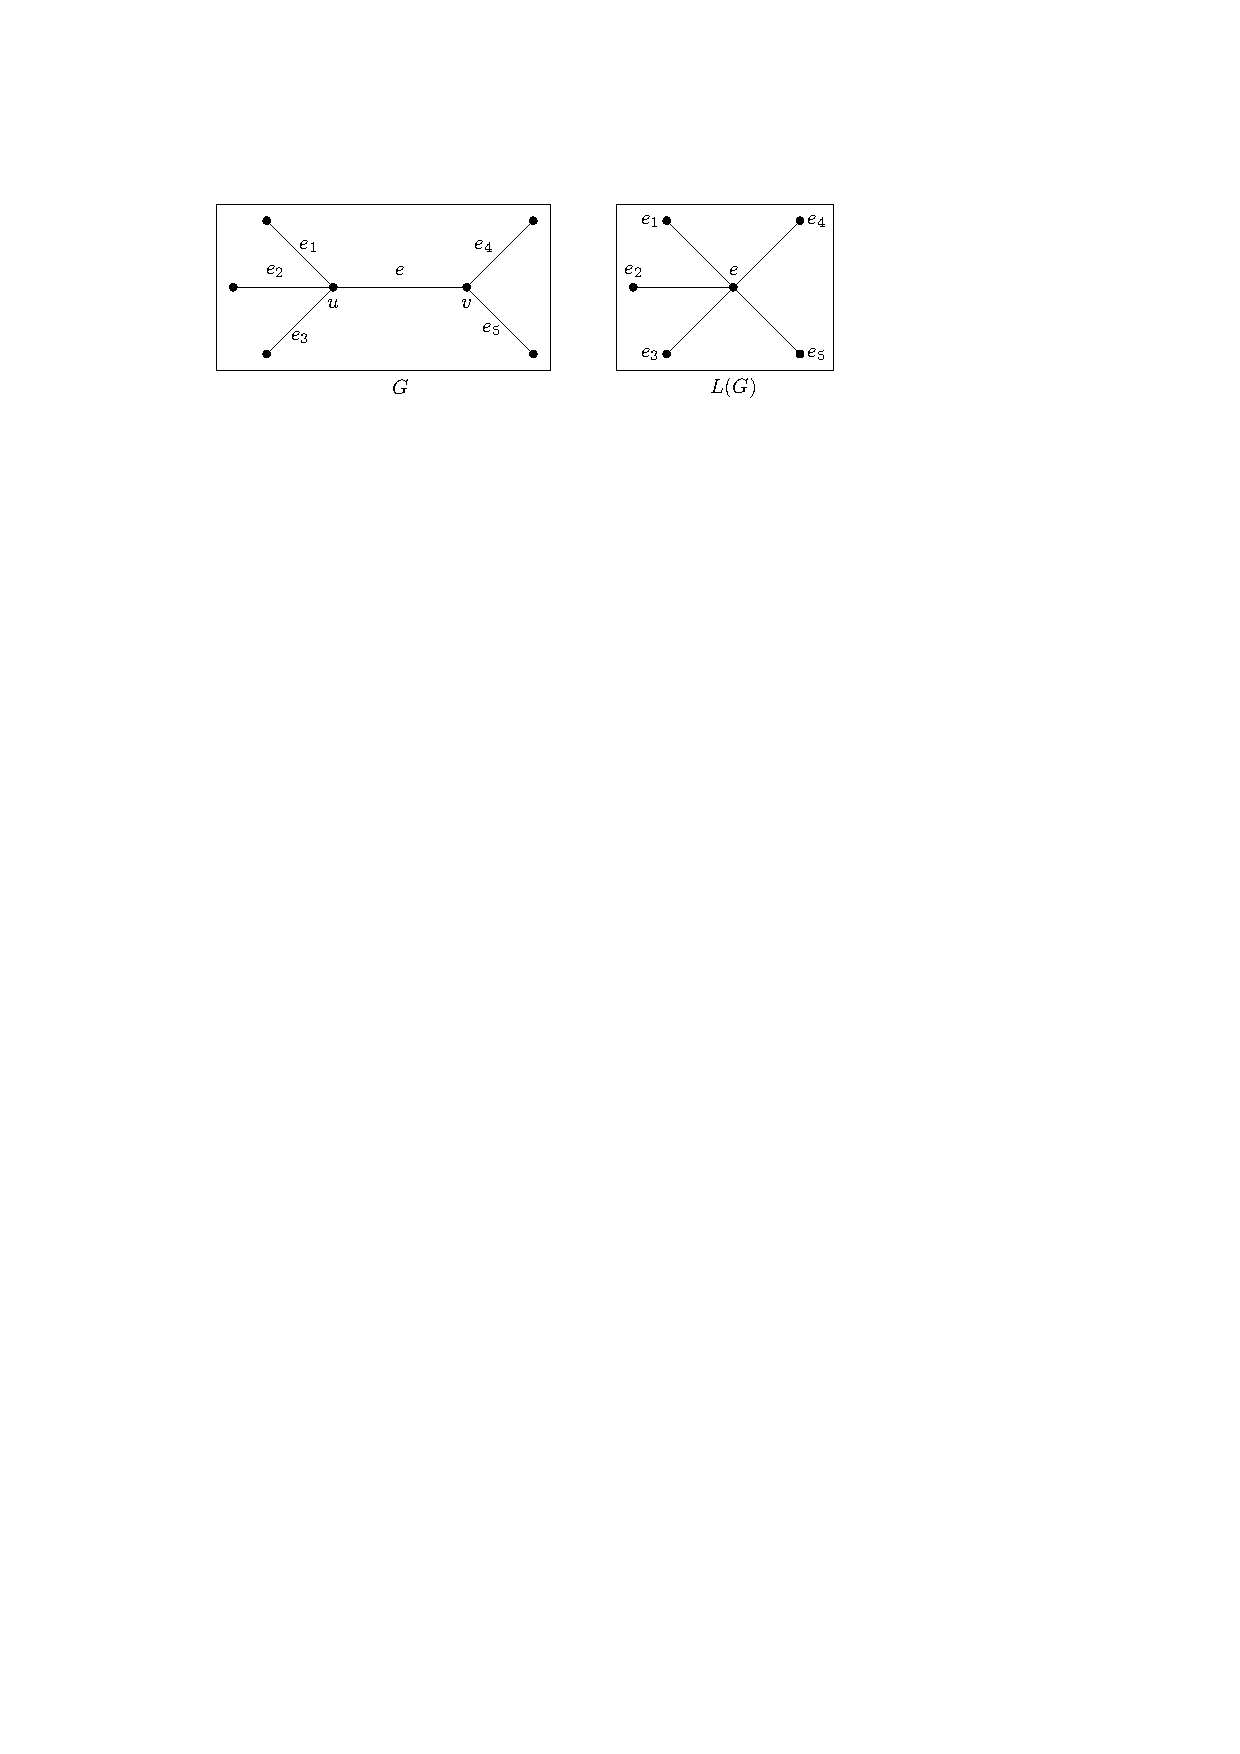
\includegraphics{Images/L(G)Neighbourhood.pdf}
\caption{Neighbourhood of a vertex in $L(G)$}
\label{fig:L(G)Neighbourhood}
\end{figure}

\begin{Theorem}
For any graph $G$ of size $m \ge 1$, its line graph $L(G)$ has order $m$ and size $\displaystyle\sum_{v \in V(G)} \binom{\deg_G v}{2}$.
\end{Theorem}

\begin{proof}
By definition, the vertices of $L(G)$ are the edges of $G$, and hence the order of $L(G)$ is the size of $G$, $m$.

Now, let $e = uv$ be an edge of $G$. In $L(G)$, $e$ is a vertex, and it is adjacent to another vertex $f$ if and only if $f$ is an edge of $G$ and is adjacent to $e$,i.e.\ $f$ is an edge of $G$ incident with one of the end vertices of $e$, namely $u$ and $v$. Thus, the degree of the vertex $e$ of $L(G)$ is equal to the total number of edges that are incident with either $u$ or $v$ in $G$, except for the edge $e$ itself.

Clearly, $u$ is incident with to $\deg_G u - 1$ edges other than $e$, and $v$ is incident with $\deg_G v - 1$ edges other than $e$. Thus, the degree of $e$ in $L(G)$ is $\deg_G u  - 1 + \deg_G v - 1$.

By Handshaking Lemma, the size of $L(G)$ is half the sum of its vertex degrees, which is
\begin{equation*}
	\frac 1 2 \sum_{uv \in E(G)} (\deg_G u - 1 + \deg_G v - 1).
\end{equation*}
As the summation is over the edges of $G$, each vertex $v$ of $G$ appears exactly $\deg v$ times in the above summation, which can therefore be written as
\begin{equation*}
	\pushQED{\qed}
	\frac 1 2 \sum_{v \in V(G)} (\deg_G v)(\deg_G v - 1) = \sum_{v \in V(G)} \binom{\deg_G v}{2}.\qedhere
\end{equation*}
\end{proof}

\fi

\subsection{Adjacency Matrices}\label{subsec:AdjMat}

The \newterm{adjacency matrix} of a graph $G$ of order $n$, with vertex set $V = \{v_1, \ldots, v_n\}$, is the $n \times n$ matrix $A = A(G)$ whose $(i,j)$-entry is
\begin{equation*}
a_{ij} = \begin{cases}
1, & v_i \sim v_j \\
0, & v_i \nsim v_j.
\end{cases}
\end{equation*}

\begin{Example}\label{ex:GNM(6-11)AdjMat}
The adjacency matrix of the graph
\begin{center}
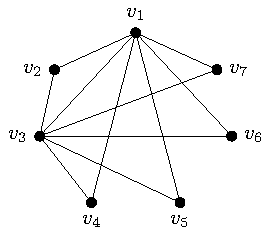
\includegraphics{Images/GNM(6,11).pdf}
\end{center}
is
\begin{equation*}
A = \begin{bmatrix}
0 & 1 & 1 & 1 & 1 & 1 & 1 \\
1 & 0 & 1 & 0 & 0 & 0 & 0 \\
1 & 1 & 0 & 1 & 1 & 1 & 1 \\
1 & 0 & 1 & 0 & 0 & 0 & 0 \\
1 & 0 & 1 & 0 & 0 & 0 & 0 \\
1 & 0 & 1 & 0 & 0 & 0 & 0 \\
1 & 0 & 1 & 0 & 0 & 0 & 0
\end{bmatrix}.
\end{equation*}
\end{Example}

Observe that, as the graphs we discuss are simple graphs and therefore have no self-loops on vertices, no vertex is adjacent to itself --i.e.\ $a_{ii} = 0$ for all $i = 1, \ldots, n$. Also, since the graphs are undirected, $v_i \sim v_j$ if and only if $v_j \sim v_i$ -- i.e.\ $a_{ij} = a_{ji}$. Thus, we have the following observation.

\begin{Observation}
The adjacency matrix of a (simple, undirected) graph is a symmetric, zero-diagonal, $(0, 1)$-matrix.
\end{Observation}

In the $i$\nth row of the adjacency matrix, for each $j$, the $j$\nth entry is $1$ if $v_j$ is adjacent to $v_i$, and $0$ otherwise. That is, the number of $1$s in the $i$\nth row is the number of vertices adjacent to $v_i$, or in other words, the degree of $v_i$. Thus, the row sums of $A$ are the vertex degrees. Observe that $A \mathbbm 1$ is the vector of row sums, where $\mathbbm 1$ is the vector (of suitable size) with all entries equal to $1$. For instance, with the matrix $A$ given in \cref{ex:GNM(6-11)AdjMat},
\begin{equation*}
A = \begin{bmatrix}
0 & 1 & 1 & 1 & 1 & 1 & 1 \\
1 & 0 & 1 & 0 & 0 & 0 & 0 \\
1 & 1 & 0 & 1 & 1 & 1 & 1 \\
1 & 0 & 1 & 0 & 0 & 0 & 0 \\
1 & 0 & 1 & 0 & 0 & 0 & 0 \\
1 & 0 & 1 & 0 & 0 & 0 & 0 \\
1 & 0 & 1 & 0 & 0 & 0 & 0
\end{bmatrix}
\begin{bmatrix}
1 \\ 1 \\ 1 \\ 1 \\ 1 \\ 1 \\ 1
\end{bmatrix} =
\begin{bmatrix}
6 \\ 2 \\ 6 \\ 2 \\ 2 \\ 2 \\ 2
\end{bmatrix}.
\end{equation*}
From the Handshaking Lemma and the preceding observation, it follows that the sum of all entries of $A$ is twice the number of edges of the graph.

\begin{Theorem}
Let $A$ be the adjacency matrix of a graph $G$ with vertex set $\{v_1, \ldots, v_n\}$. Then the $(i,j)$-entry of $A^m$, for any positive integer $m$, is the number of walks of length $m$ from $v_i$ to $v_j$.
\end{Theorem}

\begin{proof}
The $(i,j)$-entry of $A^m$ is
\begin{equation*}
(A^m)_{ij} = \sum_{1 \le k_1, \ldots, k_{m-1} \le n} a_{i k_1} a_{k_1 k_2} \cdots a_{k_{m-1} j}
\end{equation*}
Each term in this sum is $1$ if $a_{i k_1} = \cdots = a_{k_{m-1} j} = 1$ -- i.e. if $v_i \sim v_{k_1} \sim \cdots \sim v_{k_{m-1}} \sim v_j$ -- and is $0$ otherwise. Thus, each term counts a walk of length $m$ from $v_i$ to $v_j$.
\end{proof}

\begin{Theorem}
Let $A$ be the adjacency matrix of a graph $G$ with vertex set $\{v_1, \ldots, v_n\}$. Then
\begin{enumerate}[label=(\roman*)]
\item $\tr(A^2) = 2 |E(G)|$
\item $\tr(A^3) = 6 c_3(G)$
\end{enumerate}
where $c_3(G)$ denotes the number of triangles in $G$.
\end{Theorem}

\begin{proof}
We know that $(A^m)_{ij}$ is the number of walks of length $m$ from $v_i$ to $v_j$.
\begin{enumerate}[label=(\roman*)]
\item Hence, the $i$\nth diagonal entry of $A^2$, viz. $(A^2)_{ii}$, is the number of walks of length $2$ from $v_i$ to itself. Any walk of length $2$ from $v_i$ to itself is of the form $v_i v_j v_i$, where $v_j$ is a vertex adjacent to $v_i$. Thus, the number of such walks is equal to the number of vertices adjacent to $v_i$,i.e.\ $\deg v_i$. Hence, $\tr(A^2) = \sum_{i=1}^n \deg v_i = 2|E(G)|$, by Handshaking Lemma.

\item Similarly, $(A^3)_{ii}$ is the number of walks of length $3$ from $v_i$ to itself. Any such walk is of the form $v_i v_j v_k v_i$, which implies that $v_i$, $v_j$, and $v_k$ form a triangle in $G$. Moreover, each such triangle corresponds to two distinct walks from $v_i$ to itself, when traversed in the two opposite directions. Thus, $(A^3)_{ii}$ is twice the number of triangles having $v_i$ as one of its vertices. Therefore, $\tr(A^3)$ is $6 c_3(G)$, since each triangle contains three vertices, each of which counts the triangle twice in the sum $\tr(A^3)$. \qedhere
\end{enumerate}
\end{proof}

%\subsection{Incidence Matrices}\label{sec:IncMat}
%
%Consider an $(n, m)$-graph $G$ having vertex set $\{v_1, \ldots, v_n\}$ and edge set $\{e_1, \ldots, e_m\}$. The \newterm{incidence matrix} of $G$ is the $n \times m$ matrix $B = B(G)$ whose $(i, j)$-entry is $1$ if the vertex $v_i$ is incident with the edge $e_j$, and $0$ otherwise.
%
%\begin{Example}\label{ex:GNM(6-8)AdjMat}
%The incidence matrix of the graph
%\begin{center}
%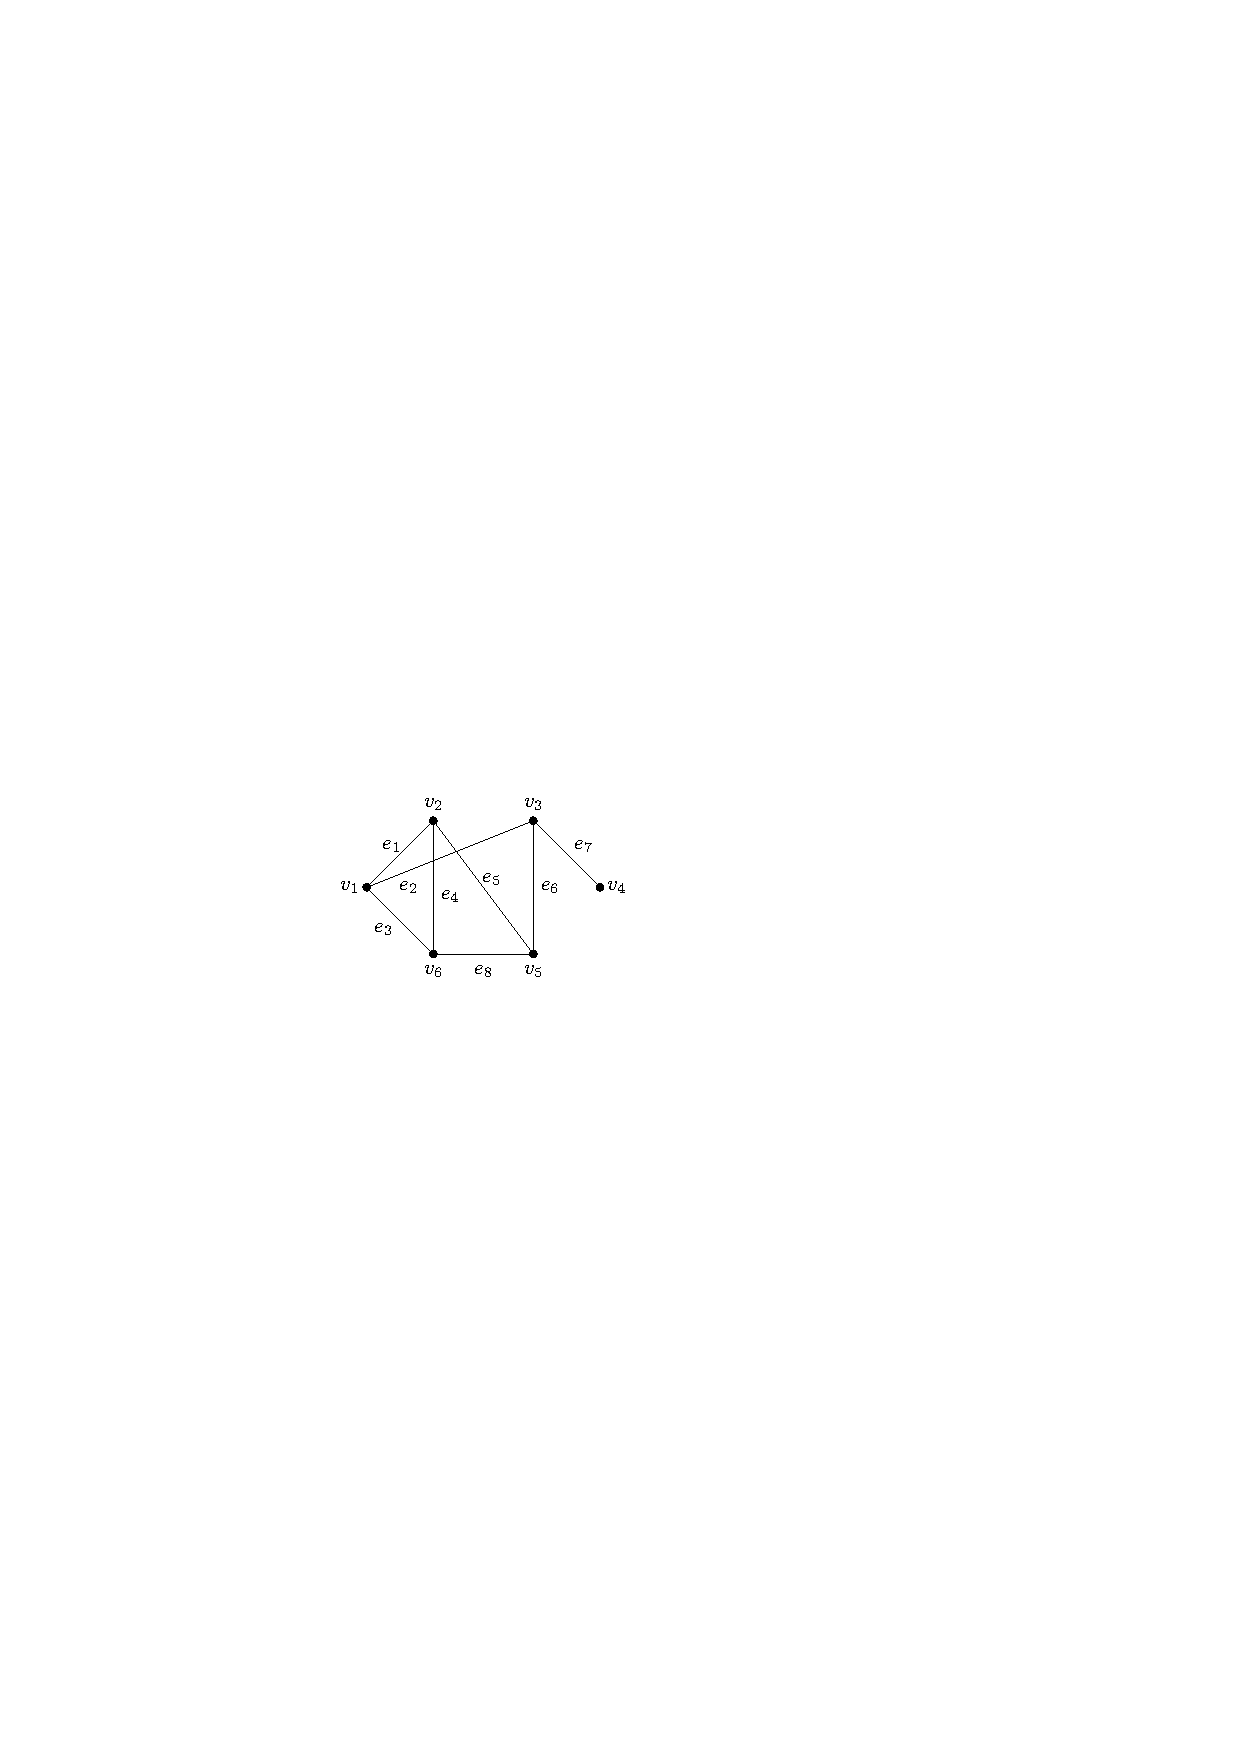
\includegraphics{Images/GNM(6,8).pdf}
%\end{center}
%is
%\begin{equation*}
%B = \begin{bmatrix}
%1 & 1 & 1 & 0 & 0 & 0 & 0 & 0 \\
%1 & 0 & 0 & 1 & 1 & 0 & 0 & 0 \\
%0 & 1 & 0 & 0 & 0 & 1 & 1 & 0 \\
%0 & 0 & 0 & 0 & 0 & 0 & 1 & 0 \\
%0 & 0 & 0 & 0 & 1 & 1 & 0 & 1 \\
%0 & 0 & 1 & 1 & 0 & 0 & 0 & 1 \\
%\end{bmatrix}.
%\end{equation*}
%\end{Example}
%
%Each column of the incidence matrix corresponds to an edge of the graph, and the only non-zero entries in the column correspond to the end-vertices of the edge -- thus, each column contains exactly two $1$s. In a simple graph, there is at most one edge between a given pair of vertices, and hence no two columns of the incidence matrix can be equal. We therefore have the following observation.
%
%\begin{Observation}
%The incidence matrix of a (simple, undirected) graph is a  $(0, 1)$-matrix in which every column has exactly two $1$s, and no two columns are equal.
%\end{Observation}
%
%\begin{Theorem}
%If $B$ is the incidence matrix of a graph $G$, then the adjacency matrix of its line graph $L(G)$ is
%\begin{equation*}
%    A\pqty{L(G)} = B^T B - 2I
%\end{equation*}
%where $I$ is the identity matrix of order $|E(G)|$.
%\end{Theorem}
%
%\begin{proof}
%Let $G$ be an $(n, m)$-graph with edge set $E = \{e_1, \ldots, e_m\}$. The incidence matrix $B = B(G)$ is of order $n \times m$, and therefore $B^T B - 2I$ (say) is of order $m \times m$.
%
%Observe that the $(i, j)$ entry of $B^T B$ is the dot product of the $i$\nth and $j$\nth columns of $B$. As each column of $B$ has exactly two non-zero entries, both equal to $1$, the $(i, i)$ entry of $B^T B$ is $2$, and therefore the diagonal entries of $B^T B - 2I$ are all zero.
%
%For $i \ne j$, the dot product of the $i$\nth and $j$\nth columns of $B$ will be $1$ if the edges $e_i$ and $e_j$ are adjacent (i.e.\ have one vertex in common), and $0$ otherwise -- note that the dot product cannot be $2$, as no two distinct columns of $B$ can be equal. Thus, for $i \ne j$, the $(i, j)$-entry of $B^T B$, which is equal to the $(i, j)$ entry of $B^T B - 2I$, is $1$ if and only if the edges $e_i$ and $e_j$ are adjacent in $G$, or equivalently, the vertices $e_i$ and $e_j$ of $L(G)$ are adjacent. Thus, $B^T B - 2I$ is the adjacency matrix of $L(G)$.
%\end{proof}

\subsection{Graph Spectra}\label{subsec:Spectra}

The \newterm{(adjacency) spectrum} of a graph is the spectrum (i.e.\ the multiset of eigenvalues) of its adjacency matrix. If the distinct eigenvalues of $A(G)$ are $\lambda_1, \ldots, \lambda_k$, with respective multiplicities $m_1, \ldots, m_k$, then we write
\begin{equation*}
\spec G = \begin{pmatrix}
\lambda_1 & \lambda_2 & \cdots & \lambda_k \\
m_1 & m_2 & \cdots & m_k
\end{pmatrix}.
\end{equation*}

\begin{Exercise}
Show that a graph $G$ of order $n$ is $k$-regular graph if and only if the all-ones vector $\mathbbm 1_n$ is an eigenvector of $A(G)$ corresponding to the eigenvalue $k$.
\end{Exercise}

\subsubsection*{Spectrum of the Complete Graph}\label{subsubsec:KnSpectrum}

The adjacency matrix of $K_n$ is $J_n - I_n$, where $J_n$ is the $n \times n$ all-ones matrix. Since the eigenvalues of $J_n$ are $n$ with multiplicity $1$ and $0$ with multiplicity $n - 1$, the spectrum of $K_n$ is
\begin{equation*}
\spec K_n = \begin{pmatrix}
n - 1 & -1 \\
1 & n - 1
\end{pmatrix}.
\end{equation*}

\begin{Exercise}
Verify that $\mathbbm 1_n$ is an eigenvector of $A(K_n)$ corresponding to the eigenvalue $n - 1$, and the column vectors $\begin{bmatrix}1 & 0 & \cdots & -1 & \cdots & 0\end{bmatrix}^T$, where the $-1$ occurs in the $i$\nth position, $i = 2, \ldots, n$, are independent eigenvectors corresponding to the eigenvalue $-1$.
\end{Exercise}

\subsubsection*{Spectrum of the Complete Bipartite Graph}\label{subsubsec:KmnSpectrum}

The spectrum of the complete bipartite graph $K_{m,n}$ is
\begin{equation*}
\spec K_{m,n} = \begin{pmatrix}
\sqrt{mn} & 0 & -\sqrt{mn} \\
1 & m + n - 2 & 1
\end{pmatrix}.
\end{equation*}

\subsubsection*{Spectrum of the Cycle}\label{subsubsec:CnSpectrum}

The eigenvalues of the cycle $C_n$, $n \ge 3$, are
\begin{equation*}
\lambda_k = 2 \cos \pqty{\dfrac{2k\pi}{n}},~ k = 0, \ldots, n - 1.
\end{equation*}

\subsubsection*{Spectrum of the Path}\label{subsubsec:PnSpectrum}

The eigenvalues of the path $P_n$ are
\begin{equation*}
\lambda_k = 2 \cos \pqty{\dfrac{k\pi}{n + 1}},~ k = 1, \ldots, n.
\end{equation*}


\subsection{Application: Centrality and Clustering}\label{subsec:Centrality}

A social network can be modelled by a graph whose vertices represent people and whose edges represent relationships or interactions. Different numerical measures capture different meanings of ``importance'', so identifying an influencer depends on the purpose of the analysis.

\subsubsection{Centrality}

Let $G$ be a connected graph of order $n \ge 2$. The following are common measures of the centrality of a vertex $v$.
\begin{enumerate}[label=(\roman*)]
\item The \newterm{degree centrality}
\begin{equation*}
    C_D(v)=\frac{\deg(v)}{n-1}
\end{equation*}
measures the proportion of the network directly connected to $v$. A large value suggests high immediate reach.

\item The \newterm{closeness centrality}
\begin{equation*}
    C_C(v)=\frac{n-1}{\displaystyle\sum_{\substack{u\in V(G)\\u\ne v}}d(u,v)}
\end{equation*}
is large when $v$ is only a few steps away from the rest of the network. Such a vertex can spread information efficiently.

\item For distinct vertices $s,t$, let $\sigma_{st}$ be the number of shortest $s$--$t$ paths and let $\sigma_{st}(v)$ be the number of these paths that pass through $v$. The \newterm{betweenness centrality}
\begin{equation*}
    C_B(v)=\sum_{\substack{\{s,t\}\subseteq V(G)-\{v\}}}
    \frac{\sigma_{st}(v)}{\sigma_{st}}
\end{equation*}
measures how often $v$ acts as a bridge between other vertices. It is particularly useful for finding brokers or potential bottlenecks.

\item An \newterm{eigenvector centrality} vector is a non-negative vector $\mathbf{x}$ satisfying
\begin{equation*}
    A\mathbf{x}=\lambda\mathbf{x},
\end{equation*}
where $A$ is the adjacency matrix and $\lambda$ is its largest eigenvalue. Its entry $x_v$ assigns a high score to $v$ when $v$ is adjacent to other high-scoring vertices.
\end{enumerate}

\begin{Remark*}
No single centrality measure always identifies the ``most influential'' vertex. Degree measures direct popularity, closeness measures rapid access, betweenness measures brokerage, and eigenvector centrality values connections to already important vertices.
\end{Remark*}

\subsubsection{Clustering (Optional)}

For a vertex $v$, let $N(v)$ be its set of neighbours and let $e(N(v))$ be the number of edges having both end-vertices in $N(v)$. The \newterm{local clustering coefficient} of $v$ is
\begin{equation*}
    C(v)=
    \begin{cases}
    \displaystyle\frac{e(N(v))}{\binom{\deg(v)}{2}},&\deg(v)\ge 2,\\[0.8em]
    0,&\deg(v)<2.
    \end{cases}
\end{equation*}
It is the proportion of pairs of neighbours of $v$ that are themselves adjacent. The \newterm{average clustering coefficient} of the network is
\begin{equation*}
    \overline C(G)=\frac{1}{n}\sum_{v\in V(G)}C(v).
\end{equation*}
A large local coefficient suggests that $v$ belongs to a tightly connected community. A vertex with high centrality but relatively low clustering may instead connect different communities.

\begin{Exercise}
For the graph in \cref{ex:GNM(6-11)AdjMat}, compute the degree and closeness centralities and the local clustering coefficient of every vertex. Which vertices would be selected as influencers by these measures?
\end{Exercise}

\begin{Exercise}
Explain how the entries of $A^2$ and $A^3$ can help detect common neighbours and triangles in a social network.
\end{Exercise}

\section{Network Reliability and Routing}\label{sec:ReliabilityRouting}

A communication, transport, or supply network may be represented by a graph. Vertices represent terminals, routers, or locations, while edges represent links or routes. Removing a vertex models the failure of a terminal and all its incident links; removing an edge models the failure of one link. This section studies structural points of failure, economical connected backbones, and shortest-path routing.

\subsection{Cutvertices, Cutedges, and Blocks}\label{subsec:Blocks}

Let $c(G)$ denote the number of components of a graph $G$. For $v \in V(G)$, the graph $G - v$ is obtained by deleting $v$ and every edge incident with it. For $e \in E(G)$, the graph $G - e$ is obtained by deleting only $e$.

A vertex $v$ is a \newterm{cutvertex} if $c(G-v) > c(G)$. An edge $e$ is a \newterm{cutedge}, or a \newterm{bridge}, if $c(G-e) > c(G)$. Thus, if $G$ is connected, a cutvertex or cutedge is one whose deletion disconnects $G$.

\begin{Theorem}\label{thm:CutedgeCycle}
An edge of a graph is a cutedge if and only if it lies on no cycle.
\end{Theorem}

\begin{proof}
Let $e = uv$. If $e$ lies on a cycle, the remaining part of that cycle is a $u$-$v$ path in $G - e$. Any path that uses $e$ can therefore be modified to avoid $e$, so deleting $e$ does not increase the number of components.

Conversely, suppose that $e$ lies on no cycle. If $u$ and $v$ were joined by a path in $G - e$, then that path together with $e$ would form a cycle containing $e$, which is not possible. Hence $u$ and $v$ lie in different components of $G - e$, and thus $e$ is a cutedge.
\end{proof}

\begin{Theorem}\label{thm:CutverChar}
If $G$ is connected and $v\in V(G)$, then the following are equivalent:
\begin{enumerate}[label=(\roman*)]
\item\label{it:CutverChar1} $v$ is a cutvertex of $G$.
\item\label{it:CutverChar2} There is a partition of $V(G) - \{v\}$ into non-empty sets $U$ and $W$ such that every $u$-$w$ path passes through $v$ whenever $u \in U$ and $w \in W$.
\item\label{it:CutverChar3} There exist vertices $u,w \in V(G) - \{v\}$ such that every $u$-$w$ path passes through $v$.
\end{enumerate}
\end{Theorem}

\begin{proof}
\cref{it:CutverChar1} $\implies $ \cref{it:CutverChar2}. Since $v$ is a cutvertex, the graph $G - v$ is disconnected, i.e.\ it has two or more components. Let $U$ be the set of all the vertices in any one of the components, and let $W$ be the set of all the remaining vertices of $G - v$. Clearly, $\{U, W\}$ is a partition of $V(G) - \{v\}$. Now, if $u \in U$ and $w \in W$, then $u$ and $w$ are in different components of $G - v$, which implies that any path from $u$ to $w$ must pass through $v$.

\noindent \cref{it:CutverChar2} $\implies$ \cref{it:CutverChar3} is obvious as the latter is a special case of the former.

\noindent \cref{it:CutverChar3} $\implies$ \cref{it:CutverChar1}. Consider the graph $G - v$. As every $u$-$w$ path passes through $v$, none of them is present in $G - v$, and therefore $G - v$ is disconnected. Hence, $v$ is a cutvertex of $G$.
\end{proof}

The following characterisation of bridges can be proved along similar lines to that of \cref{thm:CutverChar}.

\begin{Theorem}\label{thm:BridgeChar}
If $G$ is a connected graph, and $e$ is any edge of $G$, then the following are equivalent:
\begin{enumerate}[label=(\roman*)]
\item\label{it:BridgeChar1} $e$ is a bridge of $G$.
\item \label{it:BridgeChar2} $e$ is not on any cycle of $G$.
\item\label{it:BridgeChar3} There exist vertices $u$ and $w$ of $G$ such that every $u$-$w$ path contains $e$.
\item\label{it:BridgeChar4} There exists a partition of $V(G)$ into two non-empty subsets $U$ and $W$ such that for all $u \in U$ and $w \in W$, every $u$-$w$ path contains $e$. \qed
\end{enumerate}
\end{Theorem}

A \newterm{block} of a graph is a maximal connected subgraph that has no cutvertex. With this convention, each cutedge together with its end-vertices is a block isomorphic to $K_2$, and each isolated vertex is a block isomorphic to $K_1$.

\begin{Example}\label{ex:Blocks}
The graph below has six blocks and three cutvertices, namely $v_1$, $v_2$, and $v_3$.
\begin{center}
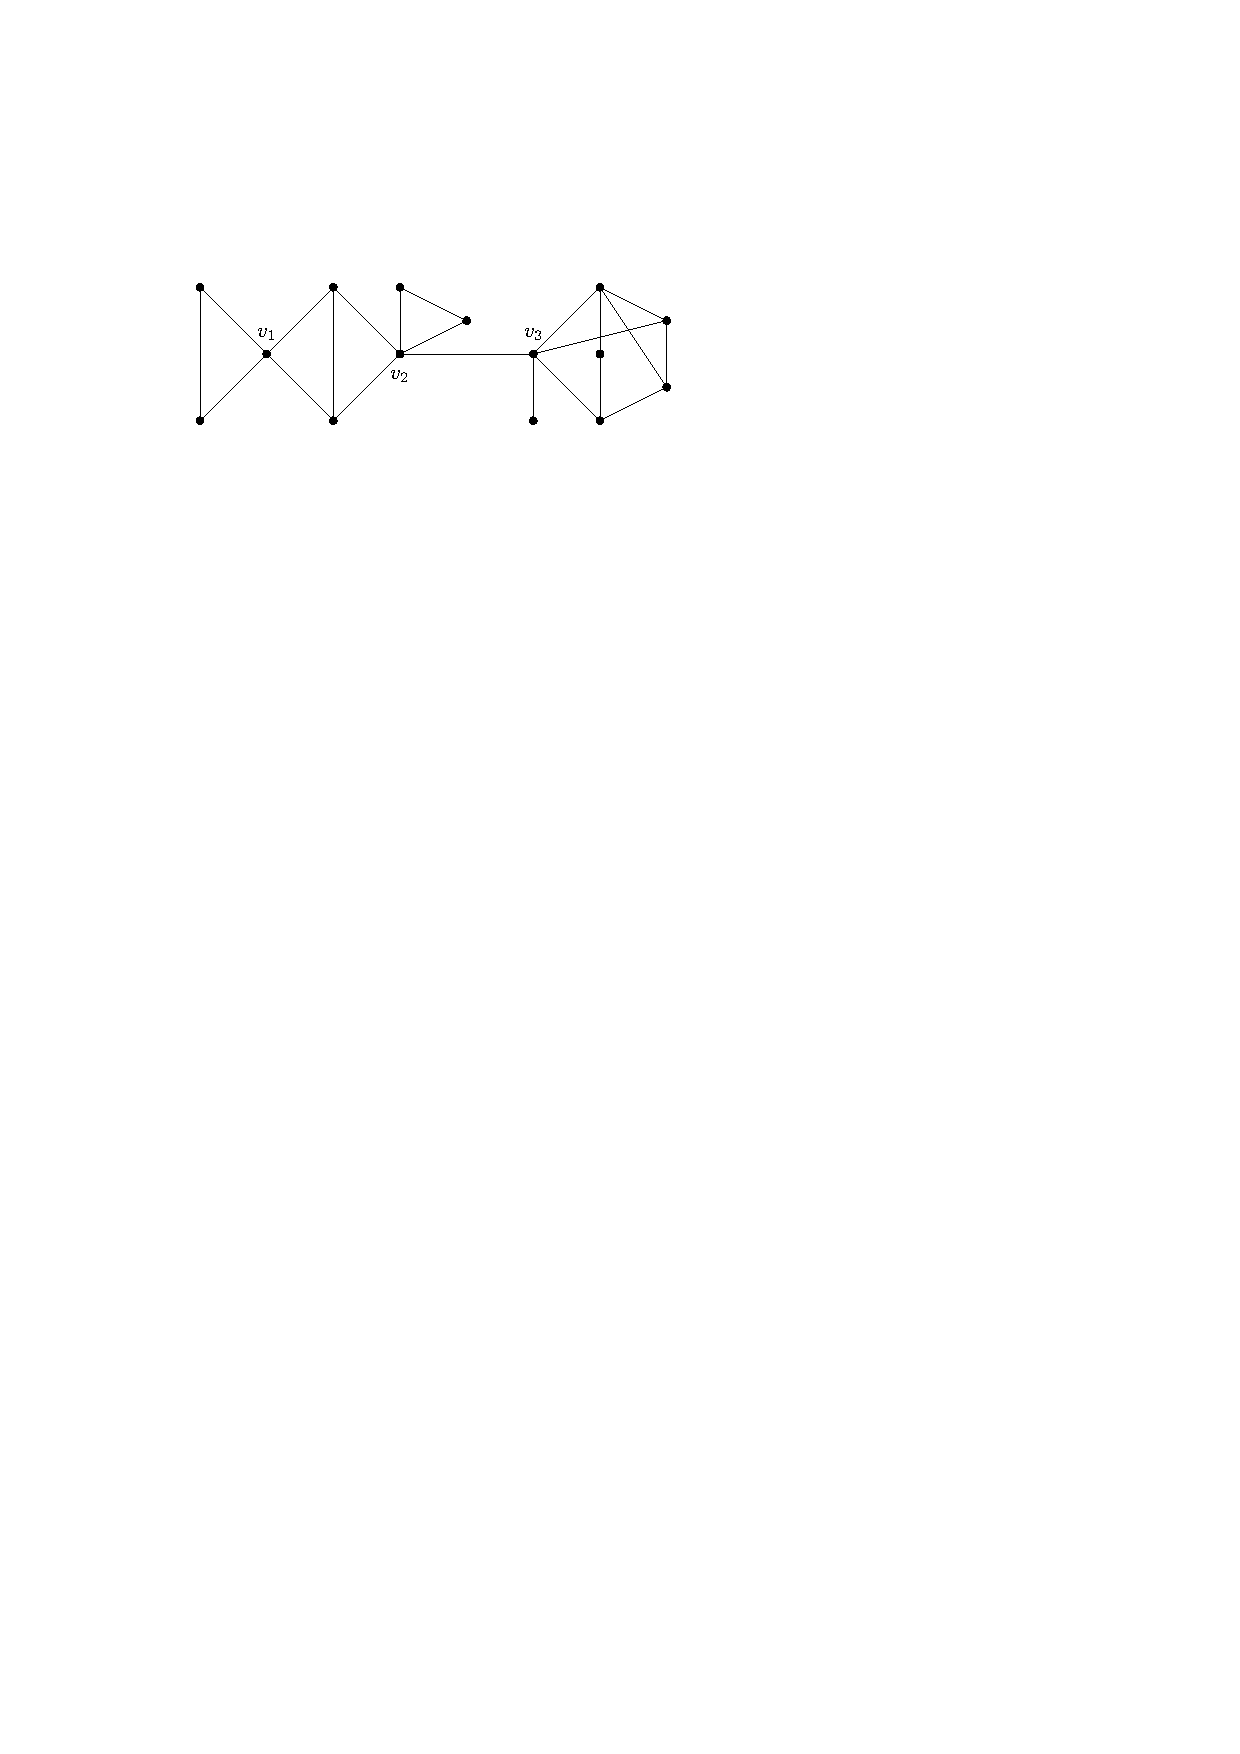
\includegraphics[width=0.68\textwidth]{Images/6BlockGraph2.pdf}
\end{center}
Its six blocks are shown separately below.
\begin{center}
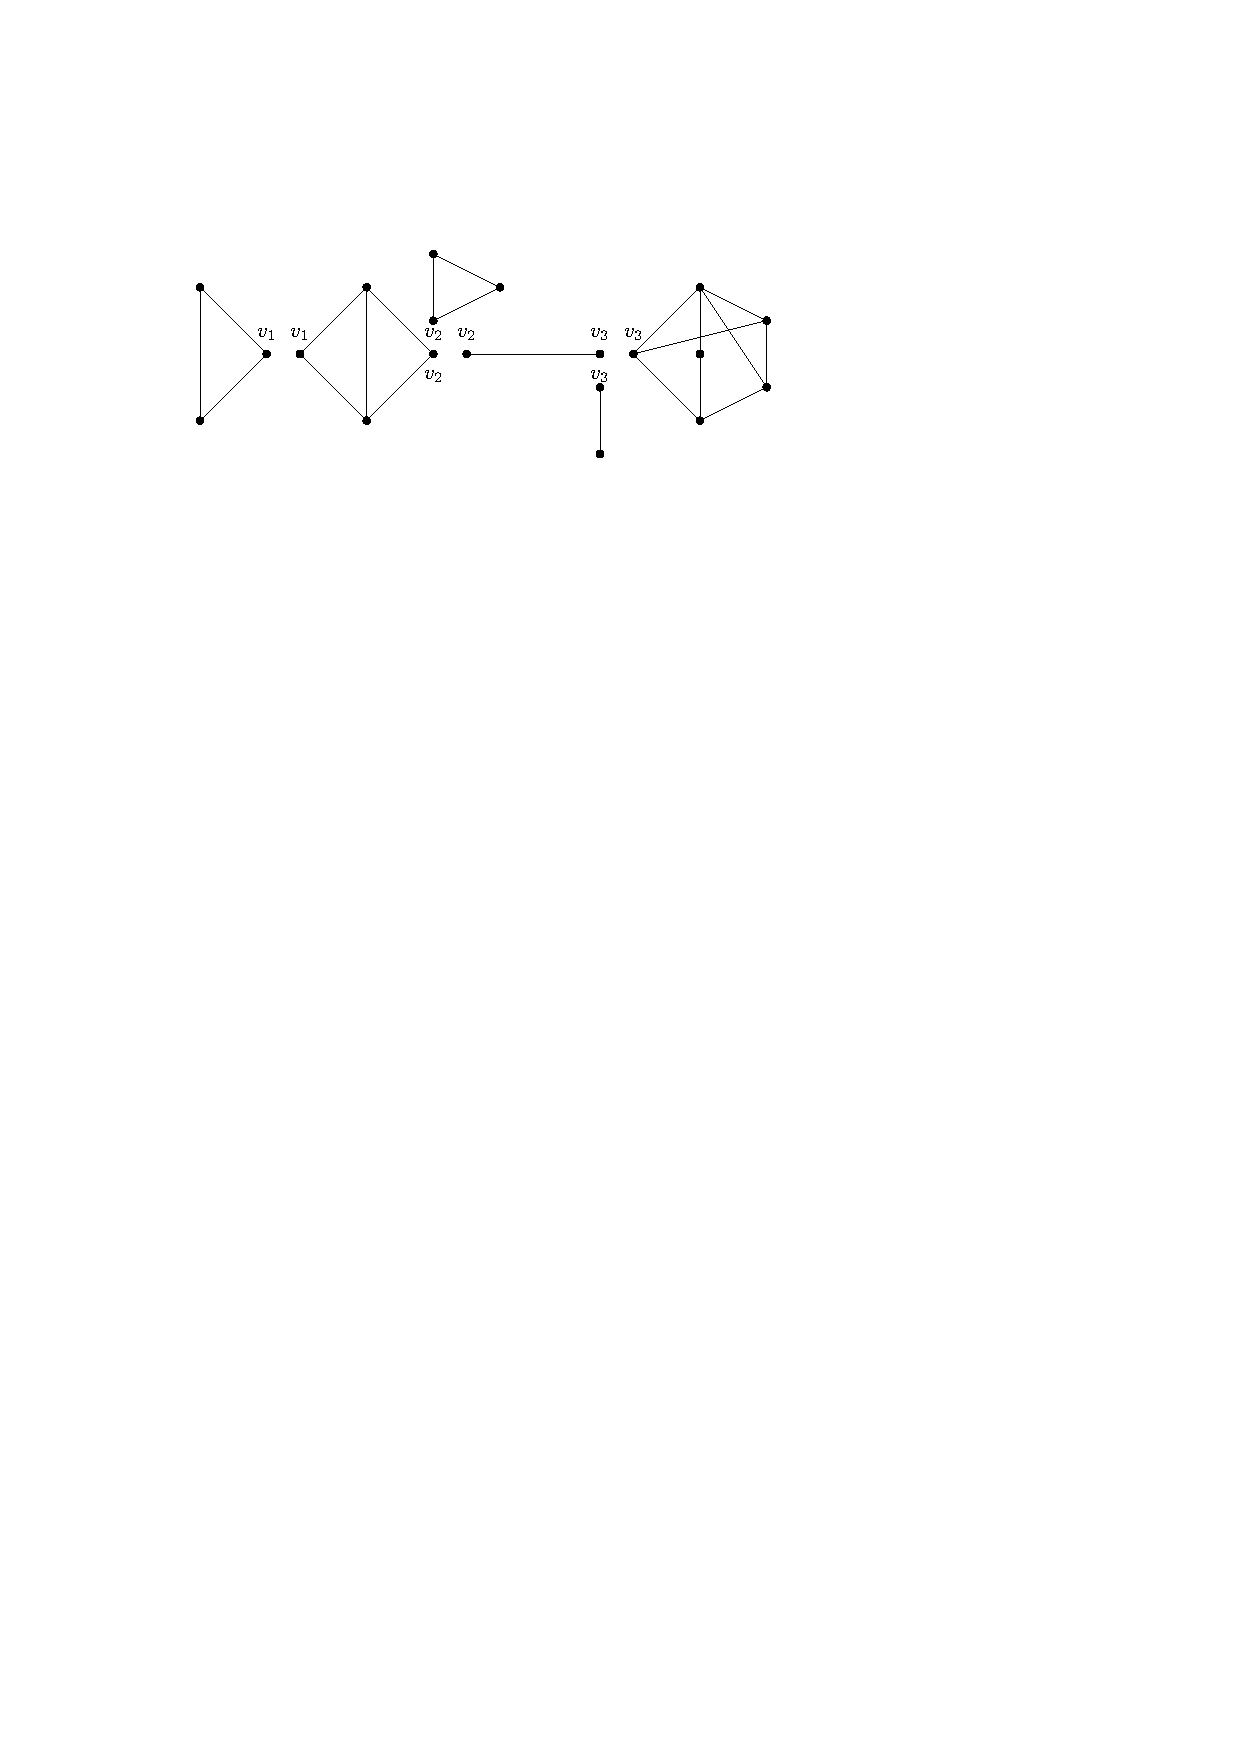
\includegraphics[width=0.9\textwidth]{Images/6BlockGraph2-Blocks.pdf}
\end{center}
\end{Example}

\begin{Theorem}\label{thm:BlockProperties}
Let $G$ be a connected graph.
\begin{enumerate}[label=(\roman*)]
\item Every edge of $G$ belongs to exactly one block.
\item Any two distinct blocks have at most one vertex in common.
\item A vertex belongs to at least two blocks if and only if it is a cutvertex. \qed
\end{enumerate}
\end{Theorem}

\begin{Theorem}\label{thm:BlockChar}
If $G$ is a connected graph of order at least $3$, then the following are equivalent:
\begin{enumerate}[label=(\roman*)]
\item\label{it:BlockChar1} $G$ is a block.
\item \label{it:BlockChar2} Every two vertices of $G$ lie on a common cycle.
\item\label{it:BlockChar3} Every vertex and edge of $G$ lie on a common cycle.
\item\label{it:BlockChar4} Every two edges of $G$ lie on a common cycle. \qed
\end{enumerate}
\end{Theorem}

The \newterm{block-cutvertex graph} of a connected graph $G$ is the bipartite graph whose vertices are the blocks and cutvertices of $G$, with a block $B$ adjacent to a cutvertex $v$ precisely when $v\in V(B)$.

\begin{Theorem}
The block-cutvertex graph of a connected graph is a tree. \qed
\end{Theorem}

\begin{Exercise}
Prove \cref{thm:BlockProperties}. Also prove that the block-cutvertex graph is a tree.
\end{Exercise}

\begin{Exercise}
Show that every edge of a tree is a cutedge, and that the cutvertices of a non-trivial tree are exactly its non-pendant vertices.
\end{Exercise}

\subsubsection{Application: Network Vulnerability Assessment}\label{subsubsec:Vulnerability}

Cutvertices and cutedges represent \newterm{single points of failure}: the failure of one such component separates terminals that could previously communicate. Blocks describe regions with no single vulnerable vertex, while the block-cutvertex tree records how these regions are joined.

The number of resulting components is only one measure of the severity of a failure. Suppose that $G$ is connected and that the components of $G-v$ have orders $s_1,\ldots,s_k$. The number of unordered pairs of surviving vertices separated by the failure of $v$ is
\begin{equation*}
    P(v)=\sum_{1\le i<j\le k}s_i s_j.
\end{equation*}
If a cutedge $e$ separates $G$ into components of orders $s$ and $n-s$, then the corresponding number of separated pairs is
\begin{equation*}
    P(e)=s(n-s).
\end{equation*}
These quantities distinguish, for example, a bridge that isolates one terminal from a bridge that divides the network into two large pieces.

\begin{Remark*}
This is a structural, deterministic model. A practical reliability assessment may also need failure probabilities, capacities, repair times, and the possibility of several simultaneous failures. Moreover, a vertex with high centrality need not be a cutvertex, and a cutvertex need not have high degree.
\end{Remark*}

\begin{Exercise}
For the graph in \cref{ex:Blocks}, determine $P(v)$ for each cutvertex and $P(e)$ for each cutedge. Rank these single points of failure from most to least disruptive.
\end{Exercise}

\subsection{Connectivity}\label{subsec:Connectivity}

For $S\subseteq V(G)$, the graph $G-S$ is obtained by deleting the vertices of $S$ and all edges incident with them. For $S\subseteq E(G)$, it is obtained by deleting the edges of $S$.

A set $S$ of vertices of a connected graph $G$ is a \newterm{separating set} or \newterm{vertex cut} of $G$ if $G - S$ is disconnected or trivial (i.e.\ a graph of order $1$). The \newterm{vertex connectivity} (or \newterm{connectivity}) of $G$, denoted by $\kappa(G)$ (or $\kappa$), is the cardinality of a minimum separating set of $G$ -- i.e.\ the minimum number of vertices of $G$ whose removal results in a disconnected or trivial graph. Similarly, a \newterm{disconnecting set} of a connected graph $G$ is a set $S$ of edges of $G$ such that $G - S$ is disconnected or trivial. The cardinality of a minimum disconnecting set of $G$ is the \newterm{edge connectivity} of $G$, and is denoted by $\lambda(G)$ (or $\lambda$). The vertex connectivity and edge connectivity of a disconnected graph are defined to be $0$.

\begin{Theorem}\label{thm:ConnectivityBounds}
For any graph $G$, $\kappa(G) \le \lambda(G) \le \delta(G)$.
\end{Theorem}

\begin{proof}
If $\delta(G) = 0$, then clearly, $\lambda(G) = 0$. If $\delta(G) \ge 1$, then disconnecting all the edges incident with a vertex of degree $\delta(G)$ disconnects $G$, and hence $\lambda(G) \le \delta(G)$.

If $G$ is disconnected, then $\kappa(G) = \lambda(G) = 0$. If $\lambda(G) = 1$, then $G$ has a bridge $e=uv$. If $G\cong K_2$, deleting either vertex leaves $K_1$. Otherwise, at least one of $u$ and $v$ is a cutvertex. Hence, in either case, $\kappa(G)=1$.

Next, let $F$ be a minimum disconnecting set of $\lambda\ge2$ edges, and choose $e=uv\in F$. By the minimality of $F$, the graph $H=G-(F-\{e\})$ is connected, while $H-e=G-F$ is disconnected. Hence, $e$ is a bridge of $H$.

For each edge of $F-\{e\}$, choose an end-vertex distinct from $u$ and $v$, and let $X$ be the set of chosen vertices. Then $|X|\le\lambda-1$, and all the edges of $F-\{e\}$ are absent from $G-X$. If $G-X$ is disconnected, then $X$ is a vertex cut. Otherwise, $e$ remains a bridge of $G-X$; deleting a suitable end-vertex of $e$ then leaves a disconnected or trivial graph. In either case, $G$ has a vertex cut of cardinality at most $\lambda$, and hence $\kappa\le\lambda$.
\end{proof}

\begin{Theorem}
For all positive integers $a$, $b$, and $c$ such that $a \le b \le c$, there exists a graph $G$ with $\kappa(G) = a$, $\lambda(G) = b$, and $\delta(G) = c$. \qed
\end{Theorem}

It is easy to see that $\kappa(K_n) = n -1$ and $\kappa(K_{p,q}) = \min(p, q)$. The $k$-dimensional \newterm{hypercube} $Q_k$ is the Cartesian product of $k$ copies of $K_2$, with $Q_0=K_1$. The following theorem gives its connectivity.

\begin{Theorem}
For any $k \ge 0$, the connectivity of the hypercube $Q_k$ is $\kappa(Q_k) = k$.
\end{Theorem}

\begin{proof}
As $Q_k$ is $k$-regular, $\kappa(Q_k)\le k$. We prove the reverse inequality by induction on $k$. The result is immediate for $k=0$ and $k=1$.

Let $k\ge2$, suppose the result holds for $Q_{k-1}$, and write $Q_k$ as two copies $G_1$ and $G_2$ of $Q_{k-1}$ joined by a perfect matching. Suppose that $S\subseteq V(Q_k)$ and $|S|\le k-1$, and put $S_i=S\cap V(G_i)$ for $i=1,2$. We show that $Q_k-S$ is connected.

If $|S_1|\le k-2$ and $|S_2|\le k-2$, then both $G_1-S_1$ and $G_2-S_2$ are connected by the induction hypothesis. At least one edge of the perfect matching has neither end-vertex in $S$, so these two subgraphs are joined in $Q_k-S$.

Otherwise, say $|S_1|=k-1$. Then $S_2=\varnothing$, so $G_2$ is intact and connected. Every surviving vertex of $G_1$ has its matching neighbour in $G_2$, and hence $Q_k-S$ is connected. Thus, no set of at most $k-1$ vertices is a vertex cut, so $\kappa(Q_k)\ge k$.
\end{proof}

\begin{Corollary}
For any $k \ge 0$, the edge connectivity of the hypercube $Q_k$ is $\lambda(Q_k) = k$.
\end{Corollary}

\begin{proof}
From \cref{thm:ConnectivityBounds}, $k = \kappa(Q_k) \le \lambda(Q_k) \le \delta(Q_k) = k$.
\end{proof}

\begin{Theorem}
If $G$ is $3$-regular, then $\kappa(G) = \lambda(G)$.
\end{Theorem}

\begin{proof}
If $G$ is disconnected, then $\kappa(G)=\lambda(G)=0$. If $G\cong K_4$, then $\kappa(G)=\lambda(G)=3$. We may therefore suppose that $G$ is connected and not complete.

Let $S$ be a minimum vertex cut of $G$. We know that $\lambda(G)\ge\kappa(G)=|S|$. The graph $G-S$ has at least two components, and the minimality of $S$ implies that every vertex of $S$ has a neighbour in every component of $G-S$.

If $G-S$ has three components, then every vertex of $S$ has exactly one neighbour in each component. The set of edges joining $S$ to any one component is therefore a disconnecting set of size $|S|$.

Now suppose that $G-S$ has two components, $H_1$ and $H_2$. A vertex of $S$ with a neighbour in $S$ has exactly one neighbour in each $H_i$; delete its edge to $H_1$. A vertex of $S$ with no neighbour in $S$ has one neighbour in one of the $H_i$ and two in the other; delete its edge to the component in which it has only one neighbour. Exactly one edge has now been deleted for each vertex of $S$, and no remaining path joins $H_1$ to $H_2$. Thus, $\lambda(G)\le|S|=\kappa(G)$, and equality follows.
\end{proof}

\subsection{Minimum Spanning Trees}\label{subsec:MST}

A \newterm{tree} is a connected graph containing no cycles. A \newterm{spanning tree} of a connected graph $G$ is a spanning subgraph of $G$ that is a tree. If every edge $e$ of $G$ has a real weight $w(e)$, the weight of a subgraph $H$ is
\begin{equation*}
    w(H)=\sum_{e\in E(H)}w(e).
\end{equation*}
A \newterm{minimum spanning tree} of $G$ is a spanning tree having minimum weight among all spanning trees of $G$.

For a non-empty proper subset $S$ of $V(G)$, the edges with one end-vertex in $S$ and the other in $V(G)-S$ form an \newterm{edge cut} of $G$.

\begin{Theorem}[Cut Property]\label{thm:CutProperty}
Let $e$ be an edge of minimum weight in an edge cut of a connected weighted graph $G$. Then some minimum spanning tree contains $e$. If $e$ is the unique minimum-weight edge in the cut, every minimum spanning tree contains $e$.
\end{Theorem}

\begin{proof}
Let the cut be determined by $S\subset V(G)$, and let $T$ be a minimum spanning tree. There is nothing to prove if $e\in E(T)$. Otherwise, adding $e$ to $T$ creates a unique cycle. As $e$ crosses the cut, this cycle contains another edge $f$ that crosses the cut. Since $e$ has minimum weight in the cut, $w(e)\le w(f)$. Replacing $f$ by $e$ therefore gives a spanning tree of weight at most $w(T)$, and hence another minimum spanning tree. If $e$ is the unique minimum-weight edge in the cut, then $w(e)<w(f)$; consequently, a minimum spanning tree omitting $e$ would not be minimum.
\end{proof}

Prim's algorithm grows a tree from an arbitrary starting vertex. At each step, it chooses a cheapest edge joining a vertex already reached to a vertex not yet reached.

\begin{algorithm}[H]\caption{Prim's algorithm}\label{alg:Prim}
\begin{algorithmic}[1]
\Require{Connected weighted graph $G$ and starting vertex $r$}
\State $S\gets\{r\}$, $F\gets\varnothing$
\While{$S\ne V(G)$}
    \State Choose a minimum-weight edge $xy$ with $x\in S$ and $y\notin S$
    \State $F\gets F\cup\{xy\}$
    \State $S\gets S\cup\{y\}$
\EndWhile
\State \Return $T=(V(G),F)$
\end{algorithmic}
\end{algorithm}

\begin{Theorem}
Prim's algorithm returns a minimum spanning tree.
\end{Theorem}

\begin{proof}
We maintain the invariant that some minimum spanning tree contains every edge in $F$. This is true initially. Suppose that a minimum spanning tree $T$ contains $F$, and let $e$ be the next edge chosen across the cut determined by $S$. If $e\in E(T)$, the invariant is preserved. Otherwise, adding $e$ to $T$ creates a unique cycle containing another edge $f$ that crosses the same cut. No edge of $F$ crosses this cut, and hence $f\notin F$. Since $e$ has minimum weight in the cut, $w(e)\le w(f)$, so $T-f+e$ is a minimum spanning tree containing $F\cup\{e\}$. Thus, the invariant is preserved.

Each iteration adds one new vertex and one edge without creating a cycle. On termination, $F$ is itself a spanning tree; since some minimum spanning tree contains all its edges, $F$ is a minimum spanning tree.
\end{proof}

\begin{Example}\label{ex:Prim}
Apply Prim's algorithm to the graph below, taking $v_1$ as the starting vertex.
\begin{center}
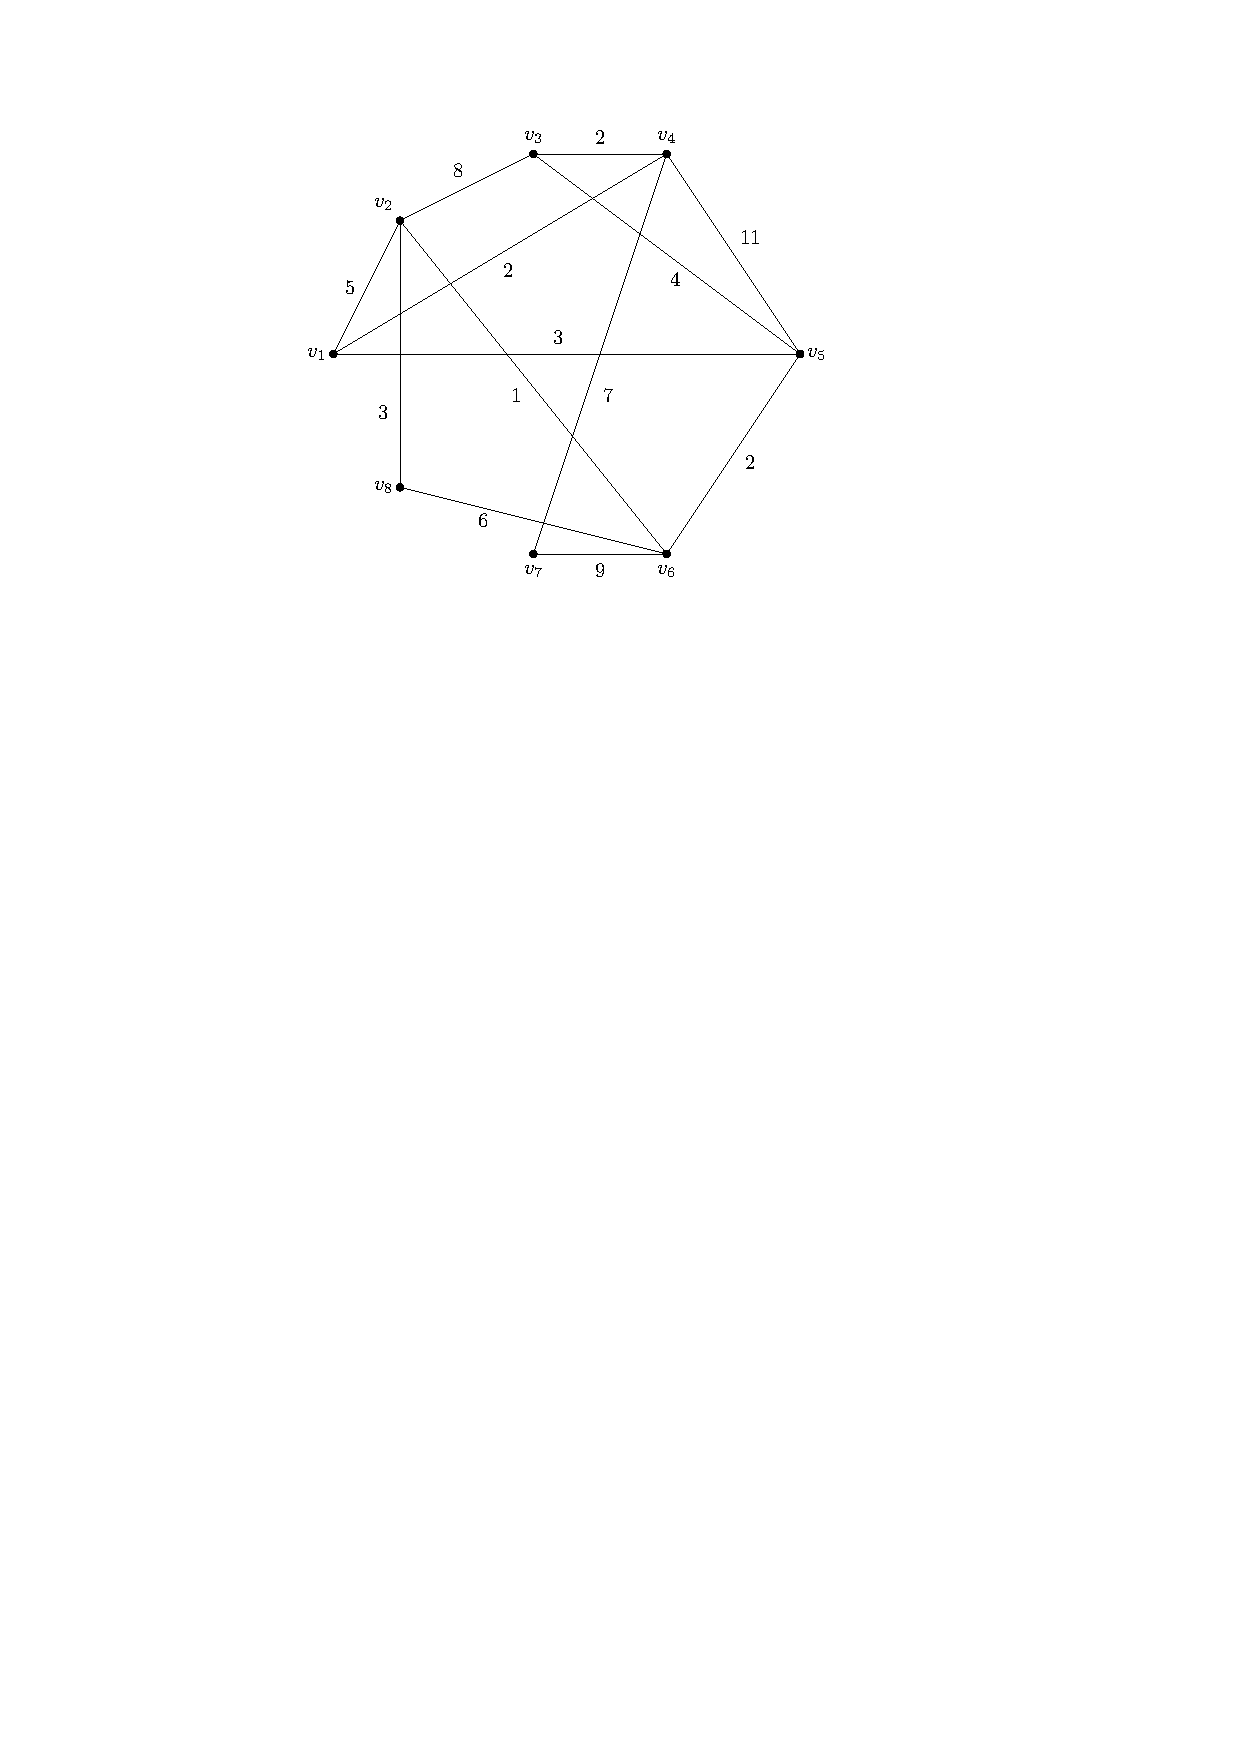
\includegraphics[width=0.55\textwidth]{Images/Prim.pdf}
\end{center}
One possible sequence of choices is shown in the table.
\begin{center}
\def\arraystretch{1.1}
\begin{tabular}{c|c|c|c}
Step & Edge added & Vertex added & Total weight \\
\hline
1 & $-$ & $v_1$ & $0$ \\
2 & $v_1v_4$ & $v_4$ & $2$ \\
3 & $v_4v_3$ & $v_3$ & $4$ \\
4 & $v_1v_5$ & $v_5$ & $7$ \\
5 & $v_5v_6$ & $v_6$ & $9$ \\
6 & $v_6v_2$ & $v_2$ & $10$ \\
7 & $v_2v_8$ & $v_8$ & $13$ \\
8 & $v_4v_7$ & $v_7$ & $20$
\end{tabular}
\end{center}
The resulting minimum spanning tree has weight $20$.
\begin{center}
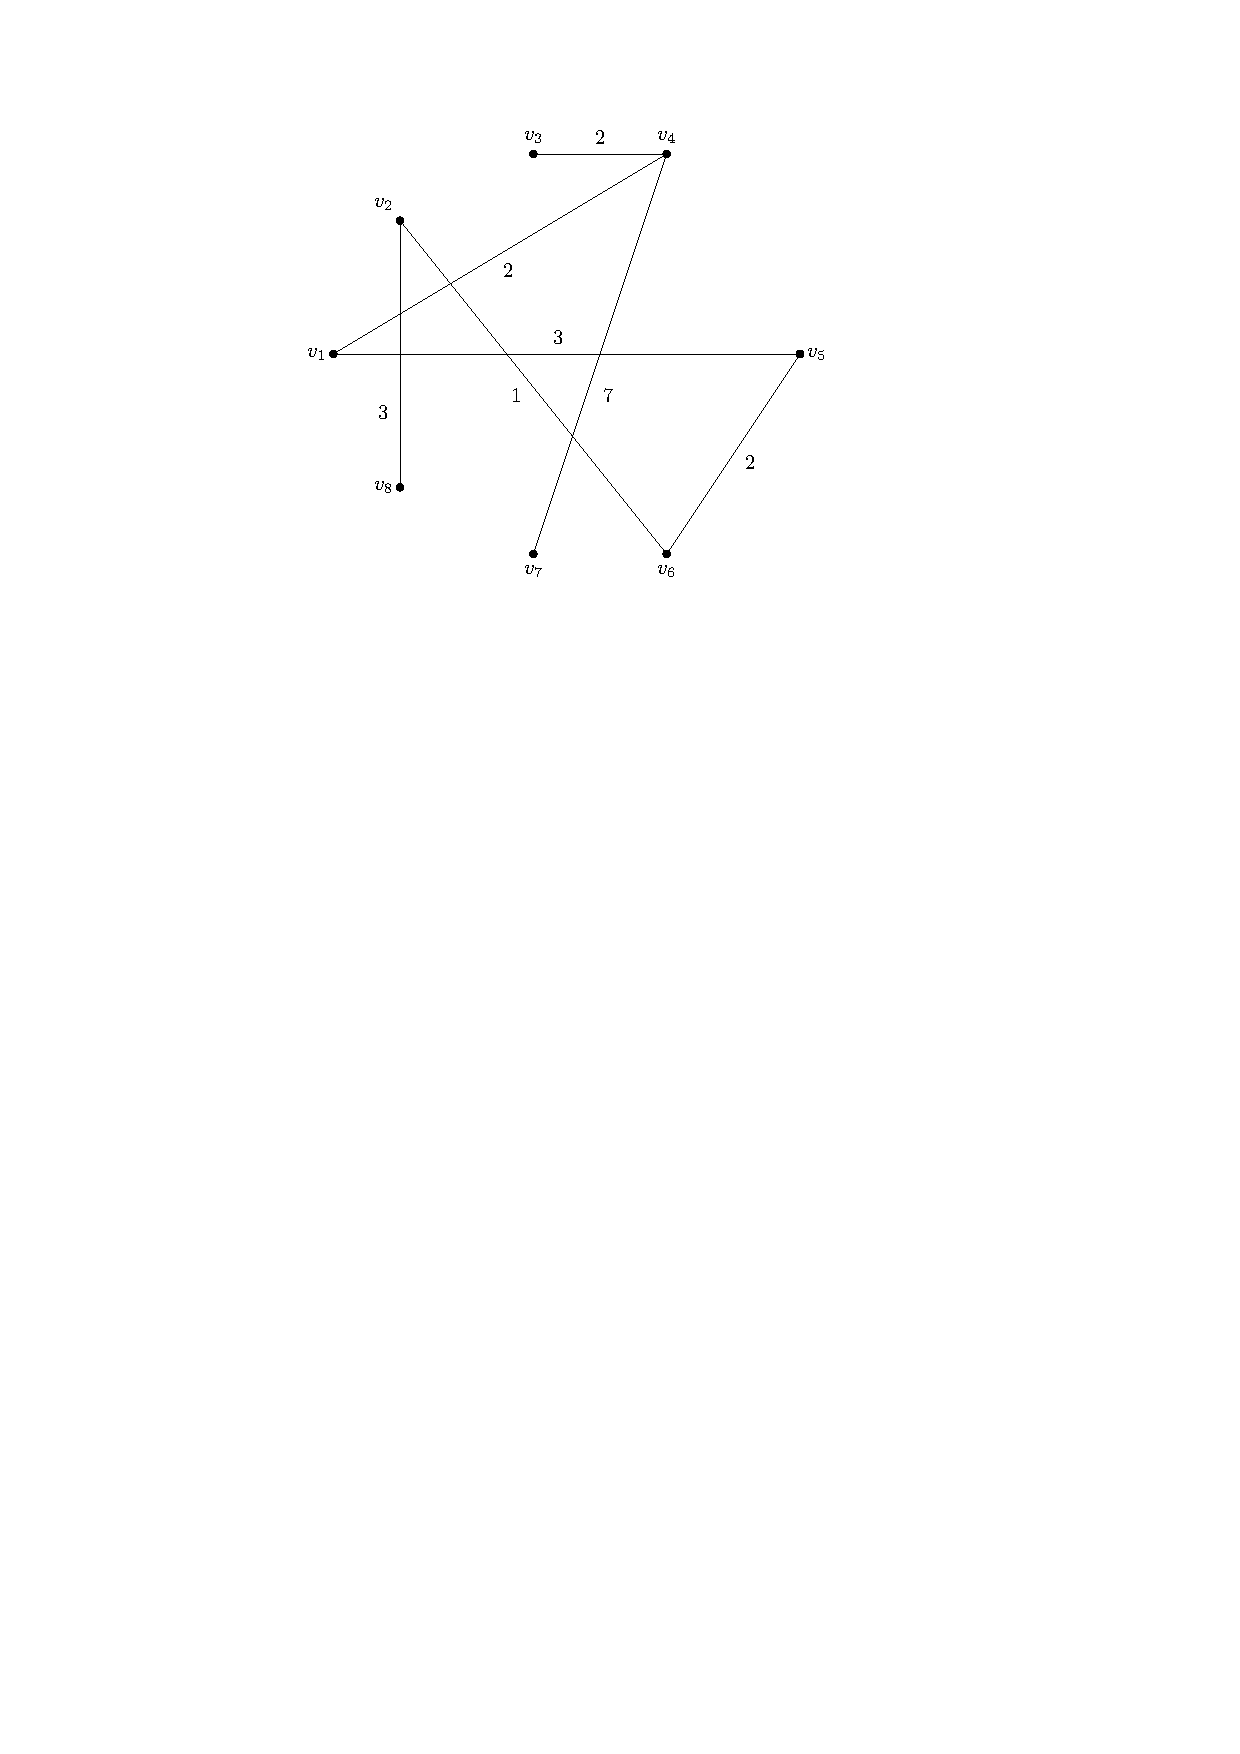
\includegraphics[width=0.56\textwidth]{Images/MST.pdf}
\end{center}
\end{Example}

\begin{Remark*}
A minimum spanning tree is a cheapest connected backbone, but it has no redundant edge: every edge of a tree is a cutedge. Cost minimisation and resilience are therefore different design objectives.
\end{Remark*}

\begin{Exercise}
Explain why Prim's algorithm can produce different minimum spanning trees when edge weights are repeated. Show that if all edge weights are distinct, the minimum spanning tree is unique.
\end{Exercise}

\subsection{All-Pairs Shortest Paths}\label{subsec:AllPairs}

Let $G$ be a weighted directed graph with vertices $v_1,\ldots,v_n$. Its \newterm{weighted adjacency matrix} is $W=(w_{ij})$, where
\begin{equation*}
w_{ij}=
\begin{cases}
0, & i=j,\\
\text{weight of the edge from $v_i$ to $v_j$}, & (v_i,v_j)\in E(G),\\
\infty, & (v_i,v_j)\notin E(G).
\end{cases}
\end{equation*}
We assume that $G$ has no negative-weight cycle. Edge weights may be negative. In the absence of a negative-weight cycle, a minimum-weight walk can always be reduced to a path. If a negative-weight cycle is reachable from $v_i$ and can reach $v_j$, however, the weights of $v_i$--$v_j$ walks are unbounded below, so there is no finite shortest-path distance from $v_i$ to $v_j$.

For $k=0,1,\ldots,n$, let $d_{ij}^{(k)}$ be the minimum weight of a $v_i$--$v_j$ path whose internal vertices belong to $\{v_1,\ldots,v_k\}$. Initially, $D^{(0)}=W$. For $k\ge1$, a shortest admissible path either avoids $v_k$, or passes through $v_k$. Therefore,
\begin{equation*}
    d_{ij}^{(k)}=\min\left\{d_{ij}^{(k-1)},
    d_{ik}^{(k-1)}+d_{kj}^{(k-1)}\right\}.
\end{equation*}
After the final stage, $d_{ij}^{(n)}$ is the distance from $v_i$ to $v_j$.

\begin{algorithm}[H]\caption{Floyd--Warshall algorithm}\label{alg:FloydWarshall}
\begin{algorithmic}[1]
\Require{Weighted adjacency matrix $W$ of order $n$}
\State $D\gets W$
\For{$k=1,\ldots,n$}
    \For{$i=1,\ldots,n$}
        \For{$j=1,\ldots,n$}
            \State $d_{ij}\gets\min\{d_{ij},d_{ik}+d_{kj}\}$
        \EndFor
    \EndFor
\EndFor
\State \Return $D$
\end{algorithmic}
\end{algorithm}

\begin{Theorem}
If $G$ has no negative-weight cycle, the matrix returned by the Floyd--Warshall algorithm is its all-pairs distance matrix.
\end{Theorem}

\begin{proof}
After iteration $k$, the entry $d_{ij}$ equals $d_{ij}^{(k)}$. This follows by induction on $k$ from the recurrence above. At $k=n$, every vertex may be used internally, so each entry is the weight of a shortest path between the corresponding vertices.
\end{proof}

The algorithm performs $n^3$ comparisons and uses an $n\times n$ matrix. Hence, its running time is $O(n^3)$ and its storage requirement is $O(n^2)$. If some diagonal entry is negative after the algorithm terminates, the graph contains a negative-weight cycle.

\subsection{Application: Routing Tables}\label{subsec:RoutingTables}

A distance matrix gives route costs but not the routes themselves. To construct routing tables, maintain a \newterm{next-hop matrix} $N$. Initially, set $N_{ij}=j$ when $(v_i,v_j)$ is an edge, and leave $N_{ij}$ undefined when $i\ne j$ and there is no such edge. Whenever the Floyd--Warshall update through $v_k$ strictly improves $d_{ij}$, also set
\begin{equation*}
    N_{ij}\gets N_{ik}.
\end{equation*}
Then $N_{ij}$ is the first vertex to visit on a shortest route from $v_i$ to $v_j$. Repeatedly consulting the appropriate row reconstructs the complete route.

\begin{Example}
Consider the weighted adjacency matrix
\begin{equation*}
W=\begin{bmatrix}
0&3&\infty&7\\
8&0&2&\infty\\
5&\infty&0&1\\
2&\infty&\infty&0
\end{bmatrix}.
\end{equation*}
Floyd--Warshall gives the distance and next-hop matrices
\begin{align*}
D&=\begin{bmatrix}
0&3&5&6\\
5&0&2&3\\
3&6&0&1\\
2&5&7&0
\end{bmatrix},\\
N&=\begin{bmatrix}
-&2&2&2\\
3&-&3&3\\
4&4&-&4\\
1&1&1&-
\end{bmatrix}.
\end{align*}
For example, the entry $N_{14}=2$ directs traffic from $v_1$ first to $v_2$. The successive next hops give the shortest route $v_1,v_2,v_3,v_4$, of total weight $6$.
\end{Example}

\begin{Exercise}
Apply Floyd--Warshall to the matrix in the preceding example, recording the matrix after each value of $k$. Verify the final distance and next-hop matrices.
\end{Exercise}

\begin{Exercise}
Suppose the weight of the edge from $v_3$ to $v_4$ in the preceding example increases from $1$ to $6$. Recompute the routing table and identify every source--destination pair whose shortest route changes.
\end{Exercise}

%\begin{appendices}
%
%\end{appendices}
